\section{PRECIPITATIONS}




IN general, the forecast of precipitations is more complicated than temperature, thus the scores are a little less good for this part especially the deterministic ones. 

    

\subsection{Deterministic Evaluation Metrics}

\subsubsection{Spearman rank correlation}

\begin{figure}[H]
\includegraphics[scale=0.3]{corr_RR_PERIOD.png}
\caption{3-months Rolling mean of Spearman Correlation in MENA Region for all centers JJA}
\end{figure}

we can show in the figure above that the best model in term of spearman correlation is the \textbf{ECMWF} center due to the great correlation in all the MENA region especially for   SON\footnote{September,October,November},JJA\footnote{June,July,August} and MAM\footnote{Mars,April,May}.

\begin{figure}[H]
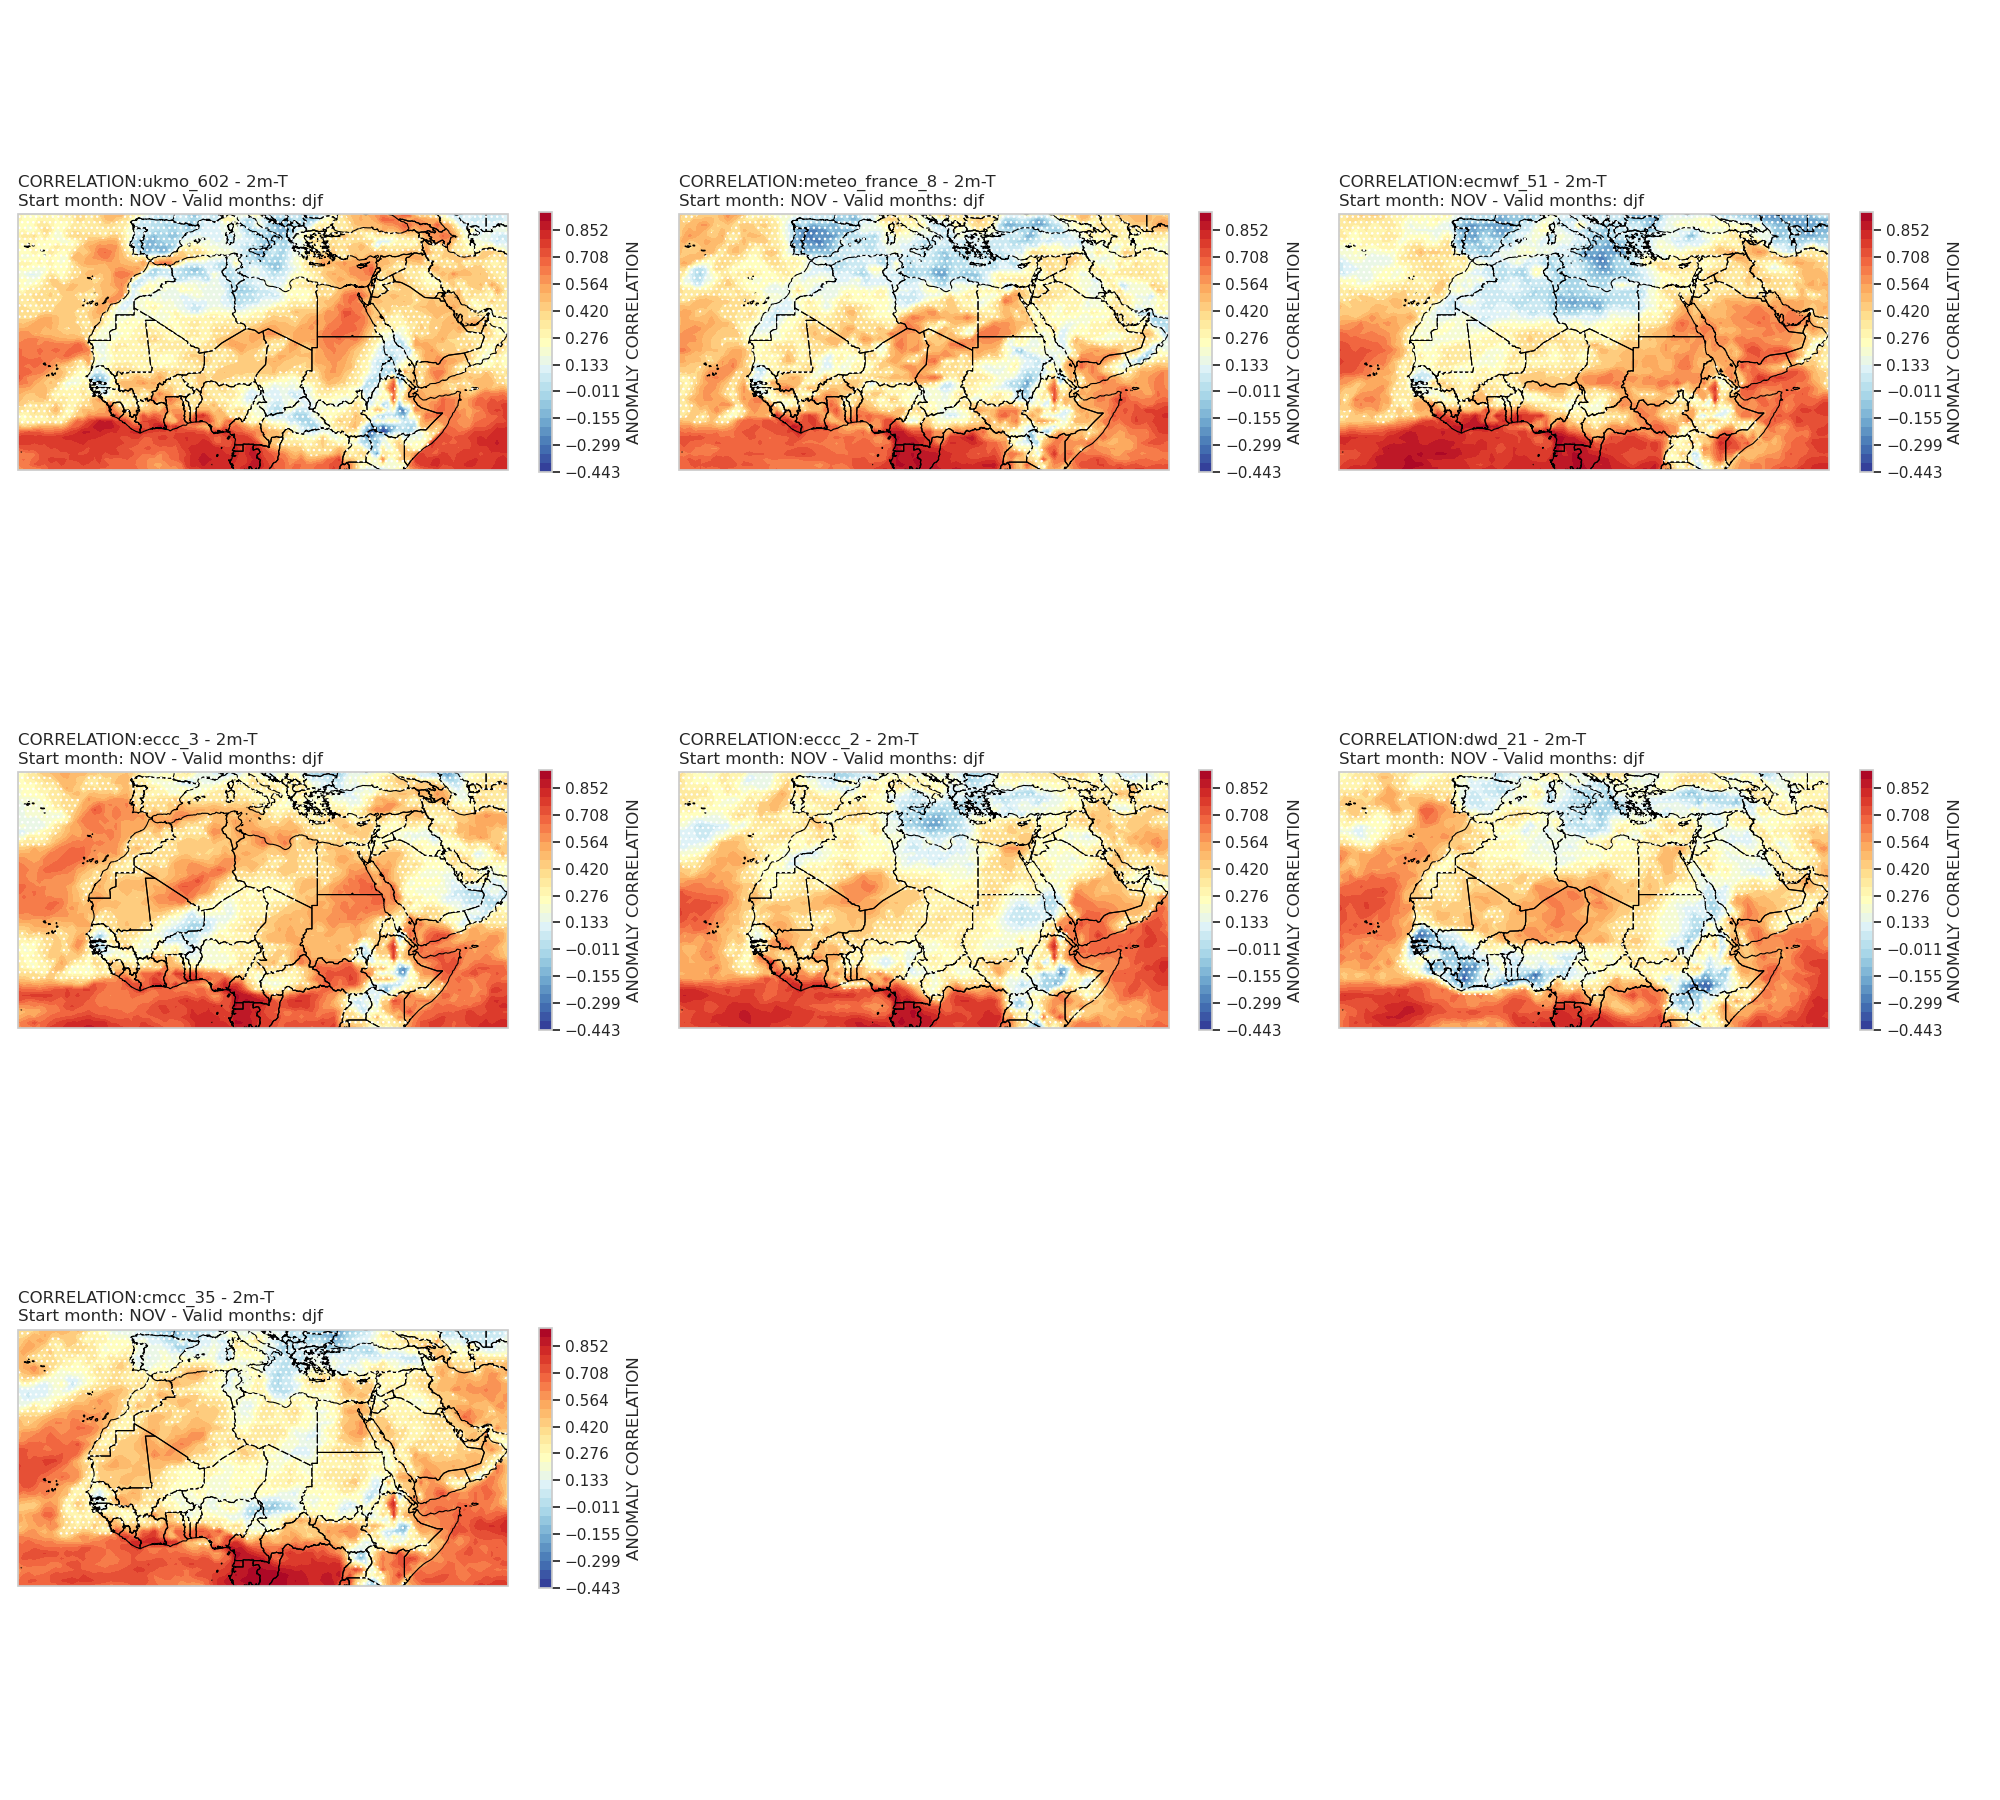
\includegraphics[scale=0.3]{CORR_DJF.png}
\caption{3-months Rolling mean of Spearman Correlation in MENA Region for all centers DJF}
\end{figure}

althought, for DJF\footnote{December,January,February} the ECMWF\footnote{European Centre for Medium-Range Weather Forecasts } , ECCC3\footnote{Environment and Climate Change Canada (ECCC) generation 3}, UKMO\footnote{UK Met Office} and CMCC 35 \footnote{Centro Euro-Mediterraneo sui Cambiamenti Climatici version 3.5} have the same performance.

\begin{figure}[H]
	\centering
	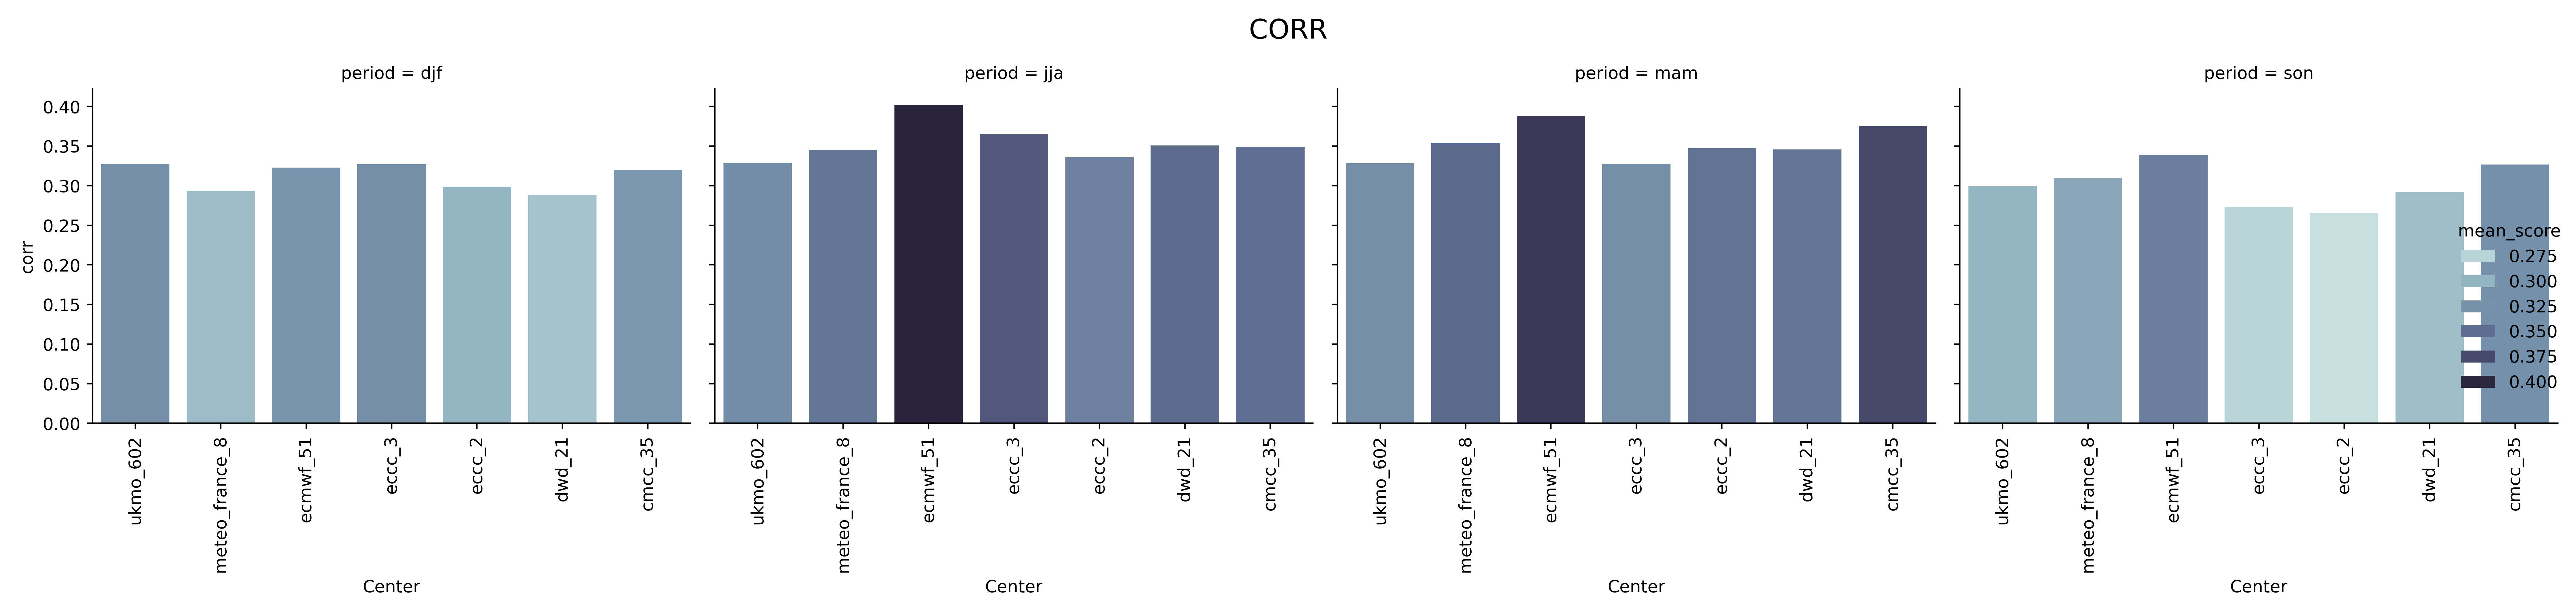
\includegraphics[scale=0.3]{corr.png}
	\caption{The average of correlation in all lead time for the mena region for every period \textbf{\textit{(1 for perfect Correlation)} }}

\end{figure}





\subsubsection{RMSE}
 
 $RMSE$ measures the average difference between a the hindcast and the observation.
 
$$RMSE=\sqrt{\frac{1}{n} \sum\limits_{i=1}^{n}(H_i -O_i)^2}$$
where :
\begin{itemize}
	\item H : the Hindcast.
	\item O : the observation.
	\item i : the valid time.
\end{itemize}

for the RMSE\footnote{Root Mean Square Error}, the Meteo-France and ECMWF have the best scores for MAM ans SON. Althought, for DJF Météo-France is better, and for JJA ECMWF is the best.

\begin{figure}[H]
\includegraphics[scale=0.3]{rmse_RR_PERIOD.png}
\caption{3-months Rolling mean of RMSE in MENA Region for all centers DJF}
\end{figure}

\begin{figure}[H]
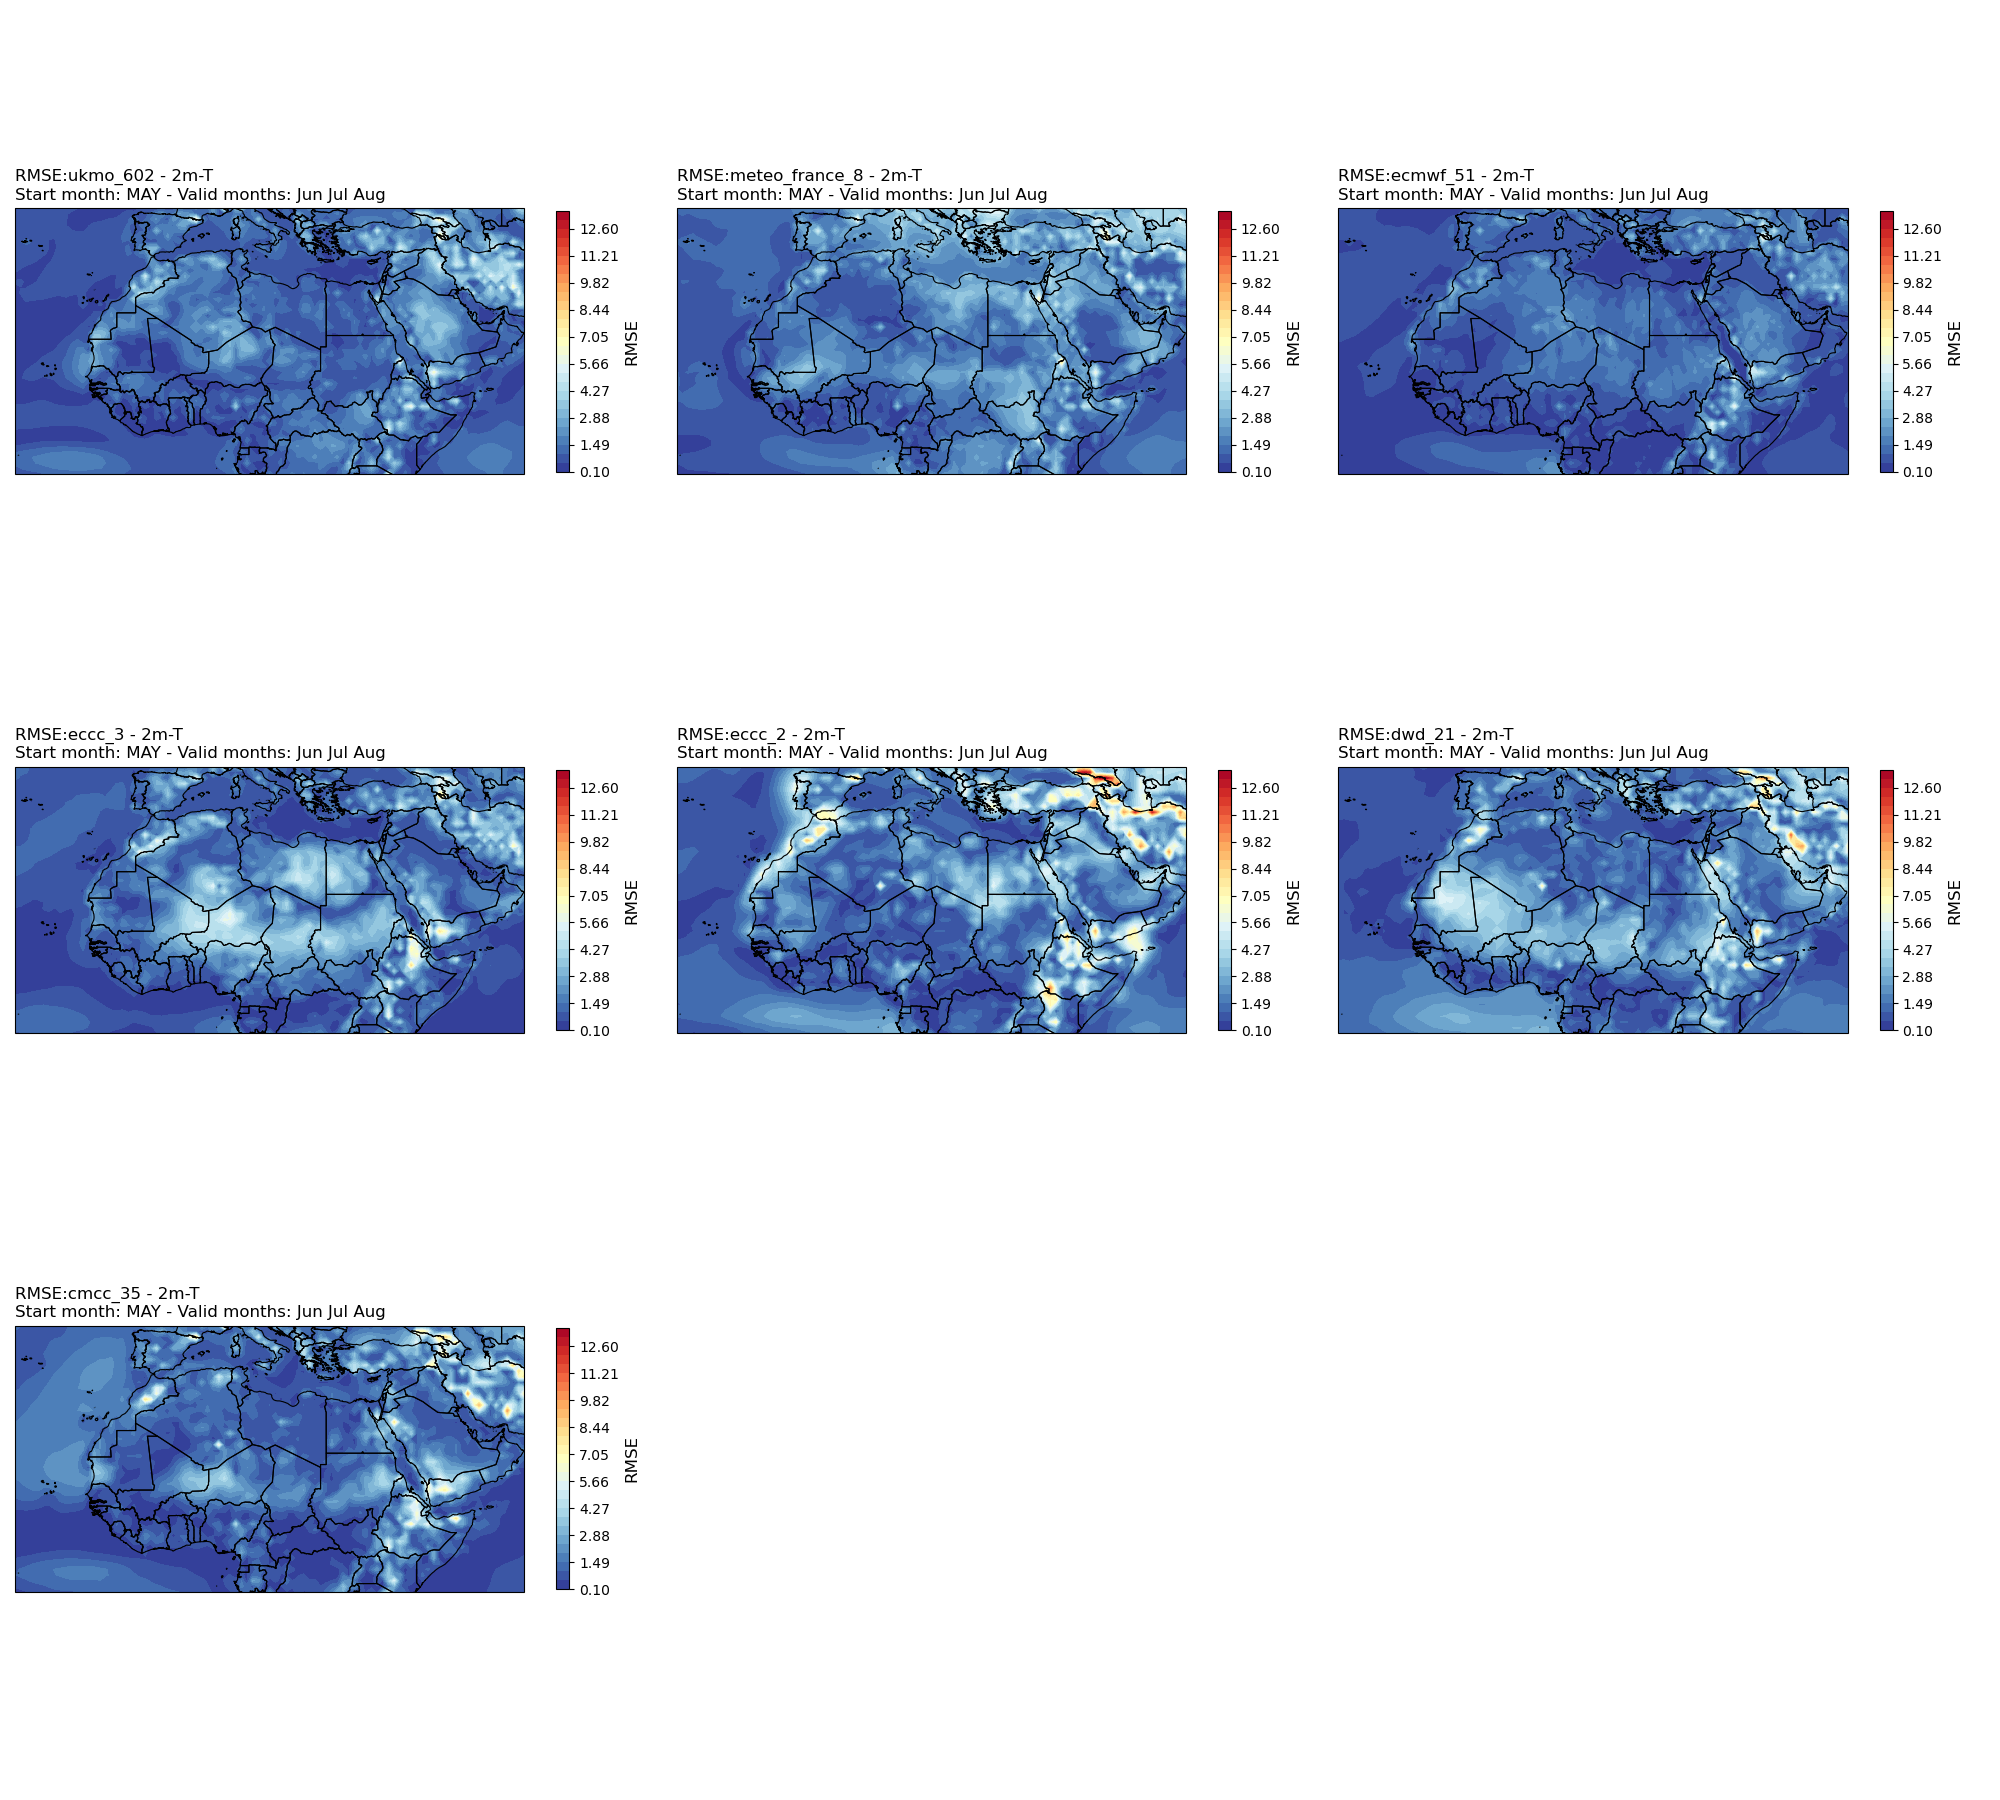
\includegraphics[scale=0.3]{RMSE_JJA.png}
\caption{3-months Rolling mean of RMSE in MENA Region for all centers JJA}
\end{figure}



\begin{figure}[H]
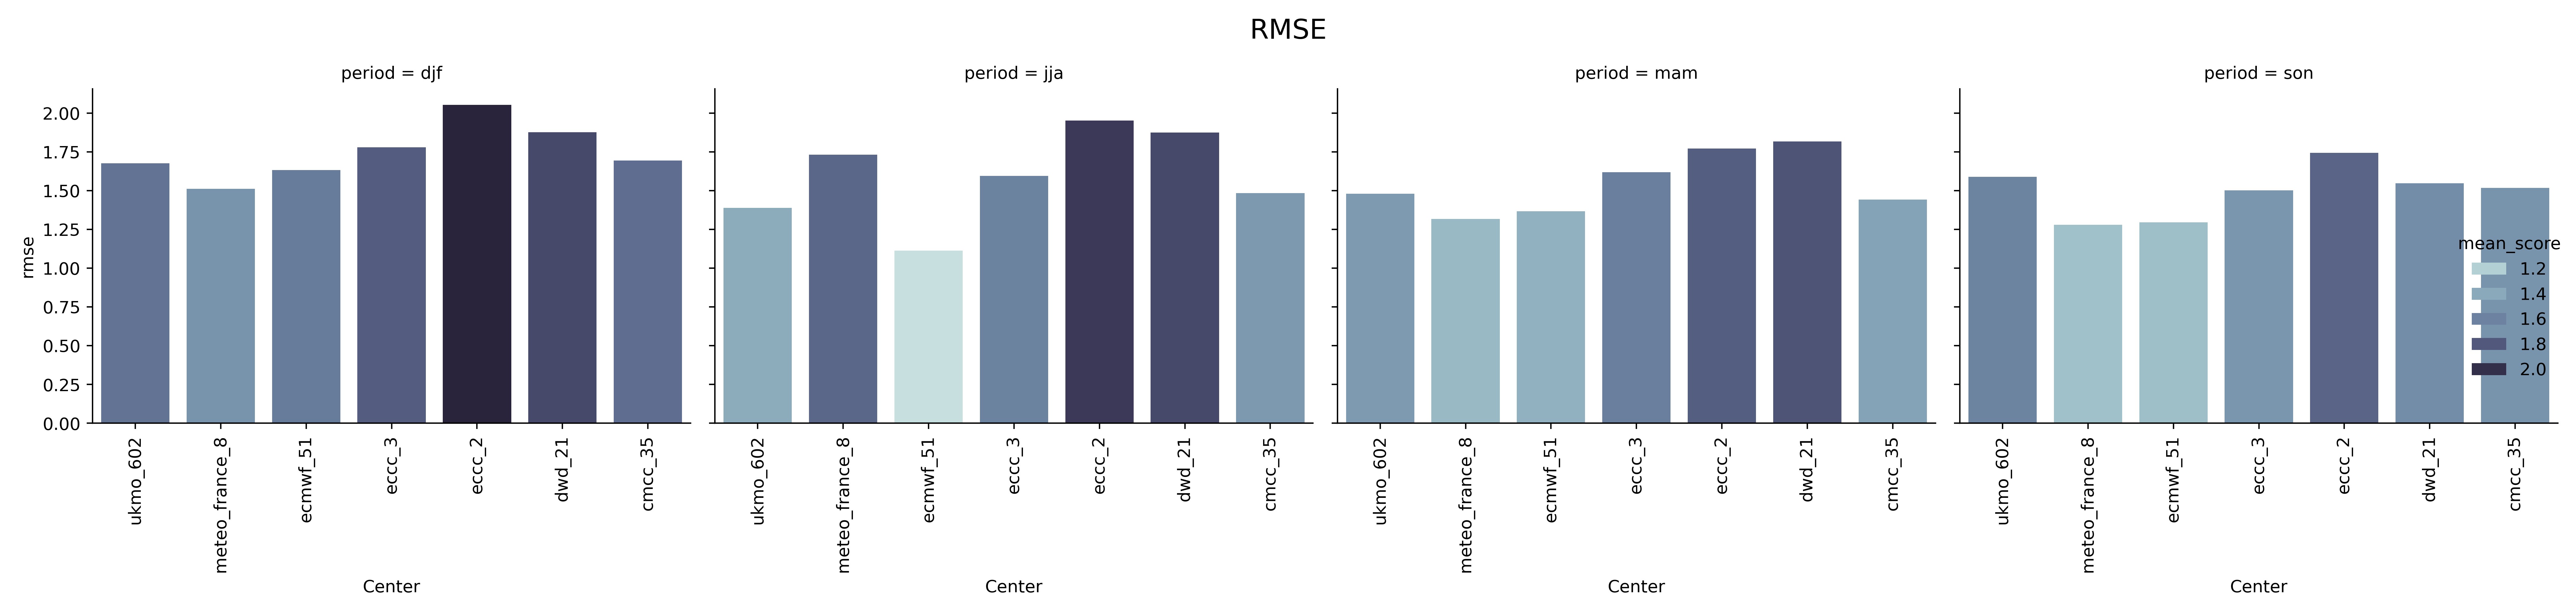
\includegraphics[scale=0.3]{rmse.png}
\caption{The average of RMSE in all lead time for the MENA region for every period \textbf{\textit{(0 for perfect RMSE)} }}
\end{figure}






\subsubsection{Coefficient of Determination (\( R^2 \))}

The coefficient of determination, \( R^2 \), is a statistical measure used to evaluate the goodness of fit of a model. It indicates the proportion of the variance in the dependent variable that is predictable from the independent variable(s). A value of \( R^2 \) close to 1 suggests that the model explains a large portion of the variance, while a value close to 0 indicates a weak relationship.

\[
R^2 = 1 - \frac{\sum_{i=1}^n (O_i - H_i)^2}{\sum_{i=1}^n (O_i - \bar{O})^2}
\]

where:

\begin{itemize}
	\item \( R^2 \): Coefficient of determination.
	\item \( H_i \): Predicted value (Hindcast).
	\item \( O_i \): Observed value (Observation).
	\item \( \bar{O} \): Mean of the observed values.
	\item \( \sum_{i=1}^n (O_i - H_i)^2 \): Residual sum of squares (unexplained variance).
	\item \( \sum_{i=1}^n (O_i - \bar{O})^2 \): Total sum of squares (total variance).
\end{itemize}

\begin{figure}[H]
\includegraphics[scale=0.3]{rsquared_RR_PERIOD.png}
\caption{3-months Rolling mean of RSQUARED in MENA Region for all centers MAM}
\end{figure}

we can show in the figure above that the best model in term of R-SQUARED is the \textbf{ECMWF} center for all periods.

\begin{figure}[H]
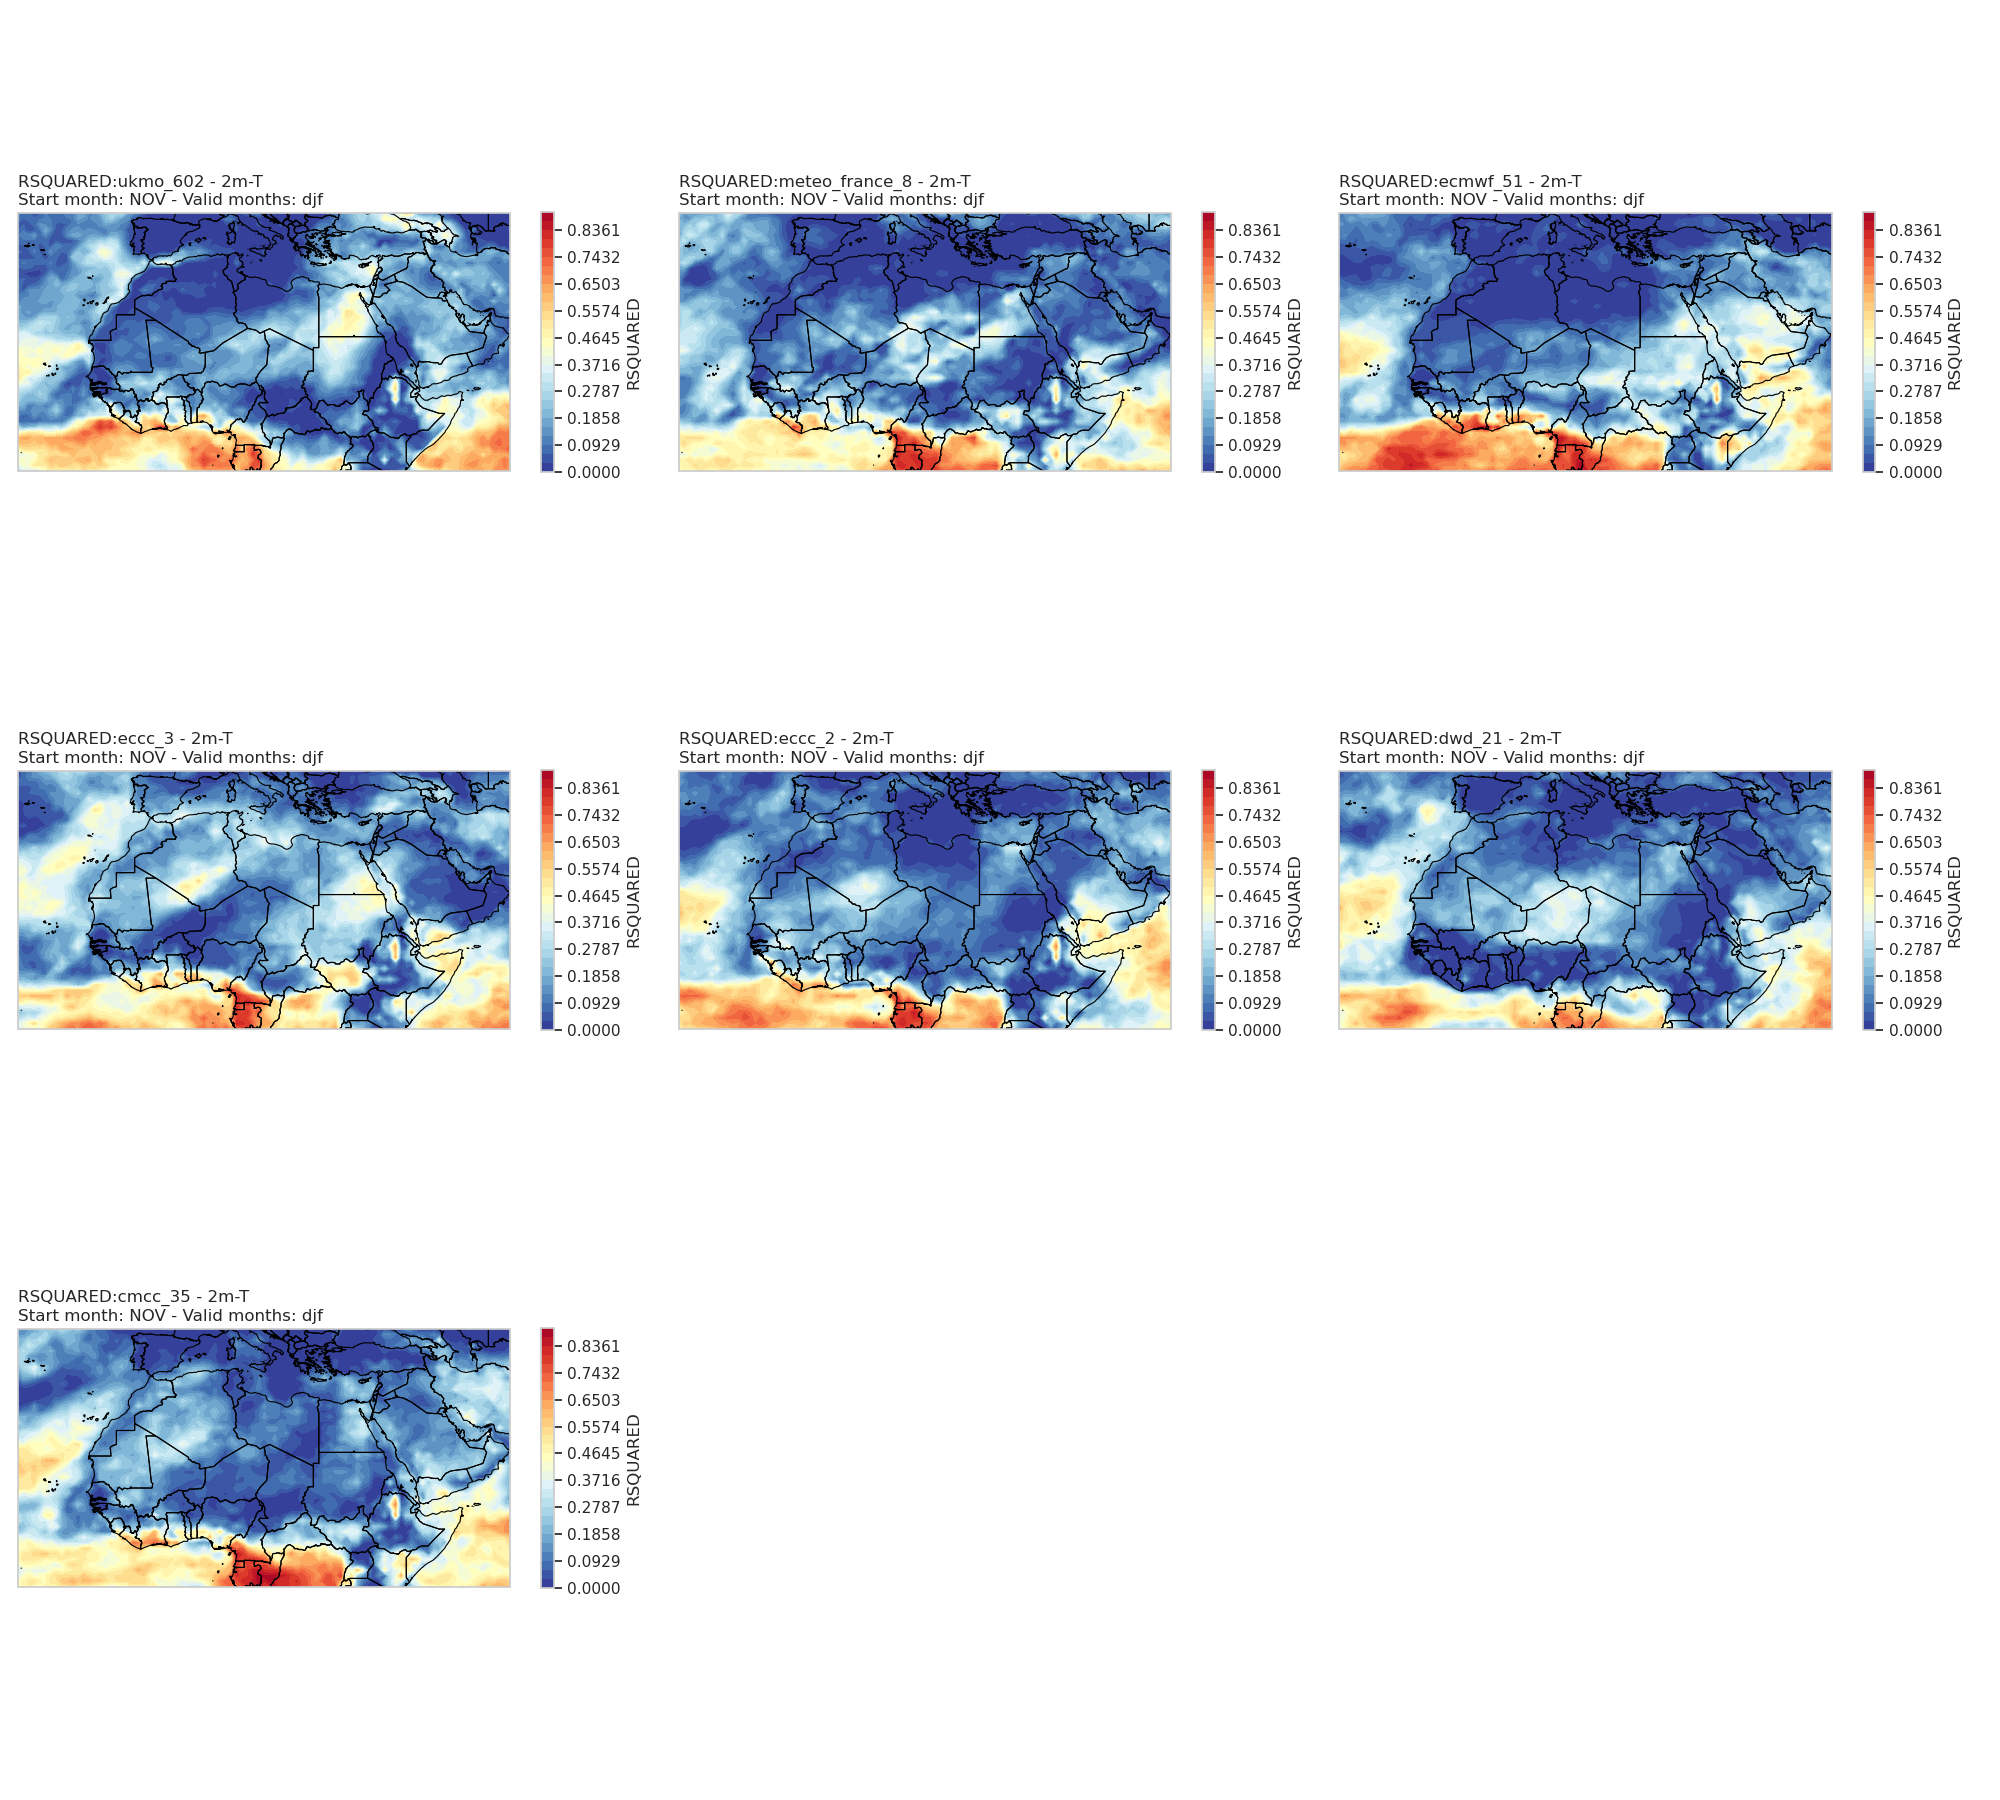
\includegraphics[scale=0.3]{RSQUARED_DJF.png}
\caption{3-months Rolling mean of RSQUARED in MENA Region for all centers DJF}
\end{figure}


\begin{figure}[H]
	\centering
	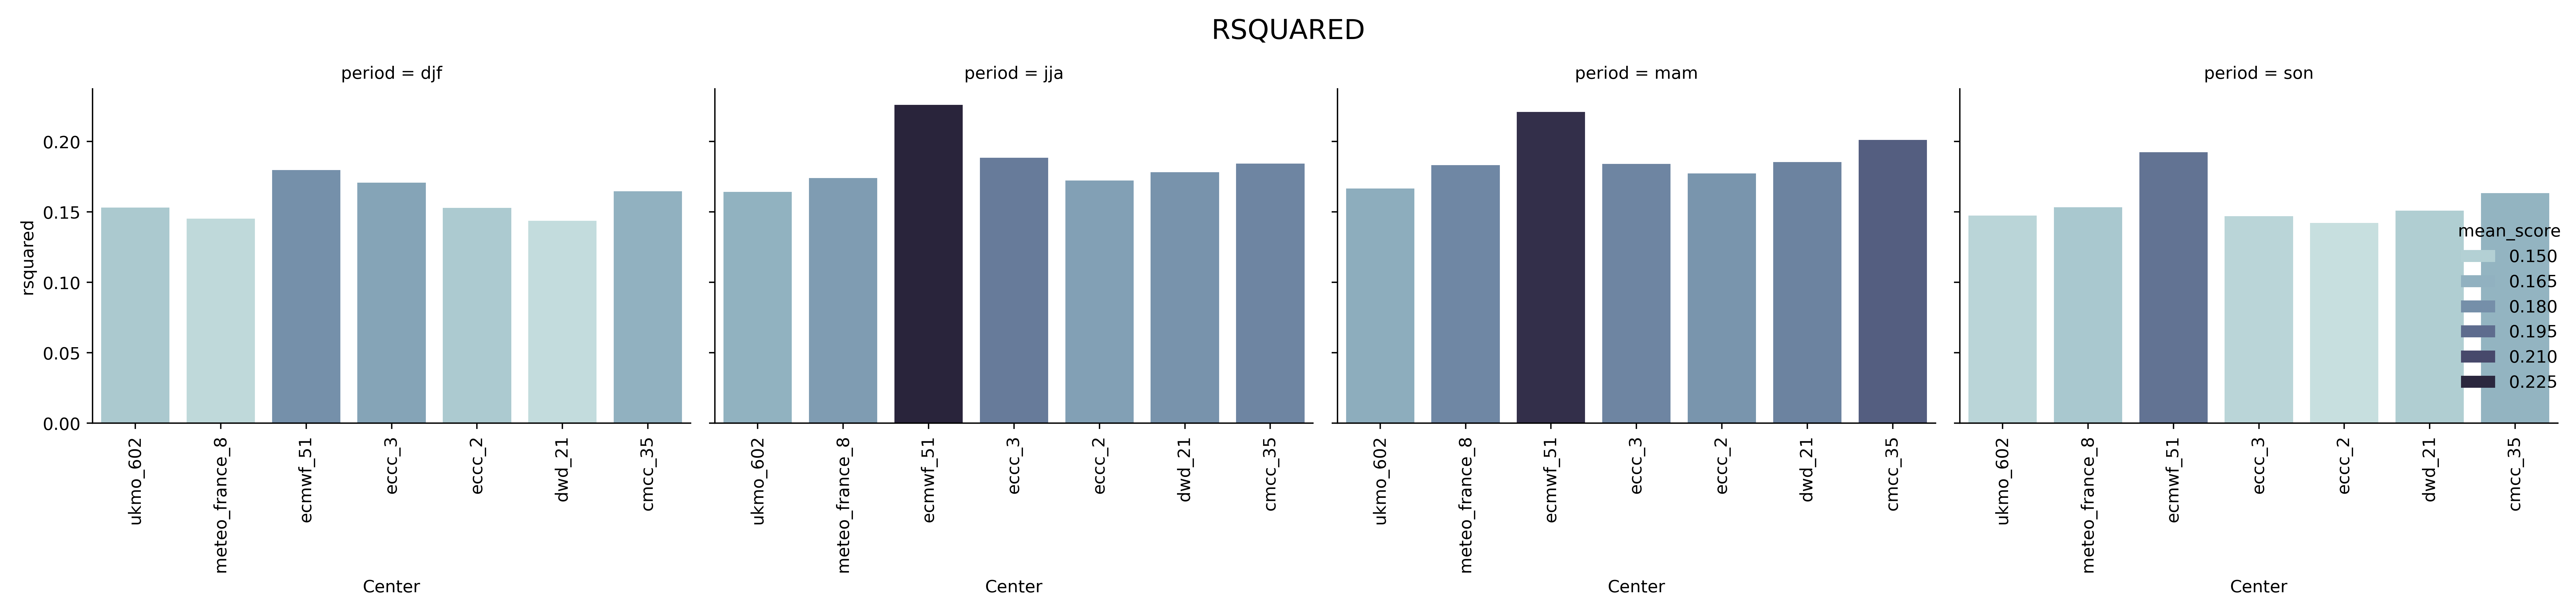
\includegraphics[scale=0.3]{rsquared.png}
	\caption{The average of rsquared in all lead time for the mena region for every period \textbf{\textit{(1 for perfect RSQUARED)} }}

\end{figure}



\subsection{Probabilistic Evaluation Metrics}

\subsubsection{The Brier Score (BS)}
The Brier Score (BS)\footnote{wmo guidance verification} is the mean squared differences between pairs of forecast probabilities p and the binary observations y. N is the total forecast number. It measures the total probability error, considering that the observation is 1 if the event occurs, and 0 if the event does not occur (dichotomous events).

$$BS_j=\frac{1}{N} \sum\limits_{i}^{N} (y_{j,i} - p_{j,i})^2$$

where:
\begin{itemize}
	\item n is the number of forecasts
	\item $y_{j,i} $ is 1 if the $i^th$ observation was in category $j$, and is 0 otherwise.
	\item $p_{j,i}$  is the $i^th$ forecast probability for category $j$.
\end{itemize}
The BS takes values in the range of 0 to 1. \textbf{\textit{Perfect forecasts receive 0}} and less accurate forecasts receive higher scores. Under the condition that x is 0.5 when the observation data is uncertain, the mean squared differences between the forecast probabilities and observation at 0.5 is calculated.


\begin{figure}[H]
    \centering
    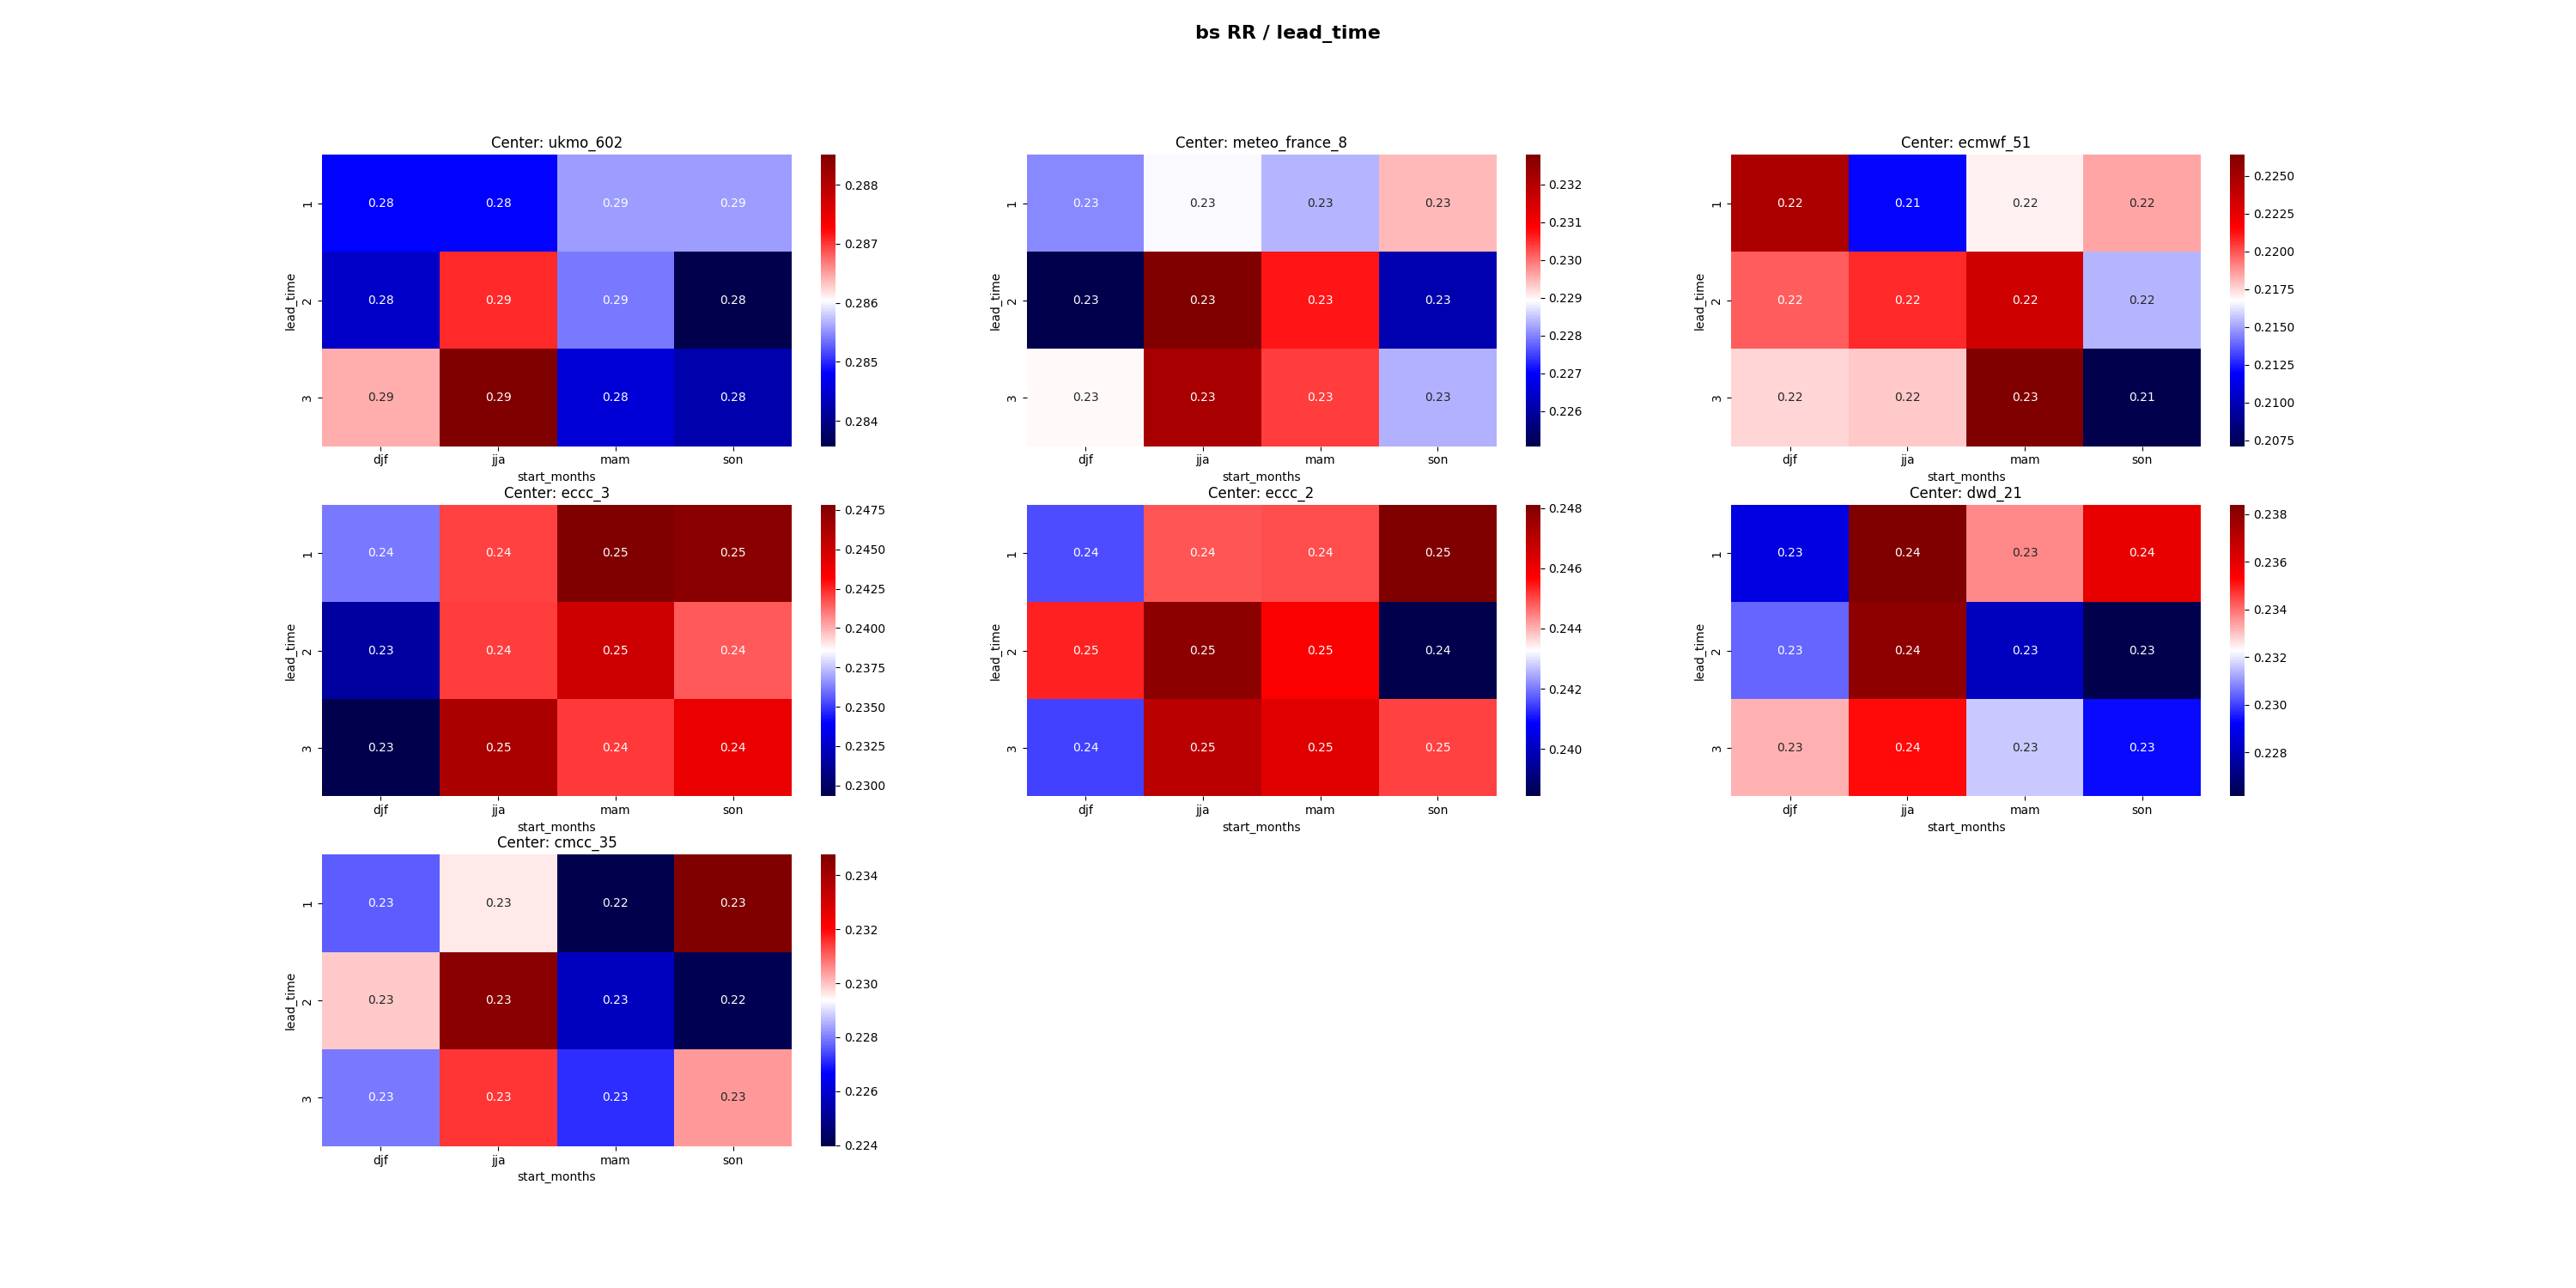
\includegraphics[scale=0.3]{bs_RR_lead_time.png}
    \caption{The Brier Score for each category  . \textbf{\textit{(0 represents perfect BS)}}}
\end{figure}

\begin{figure}[H]
    \centering
    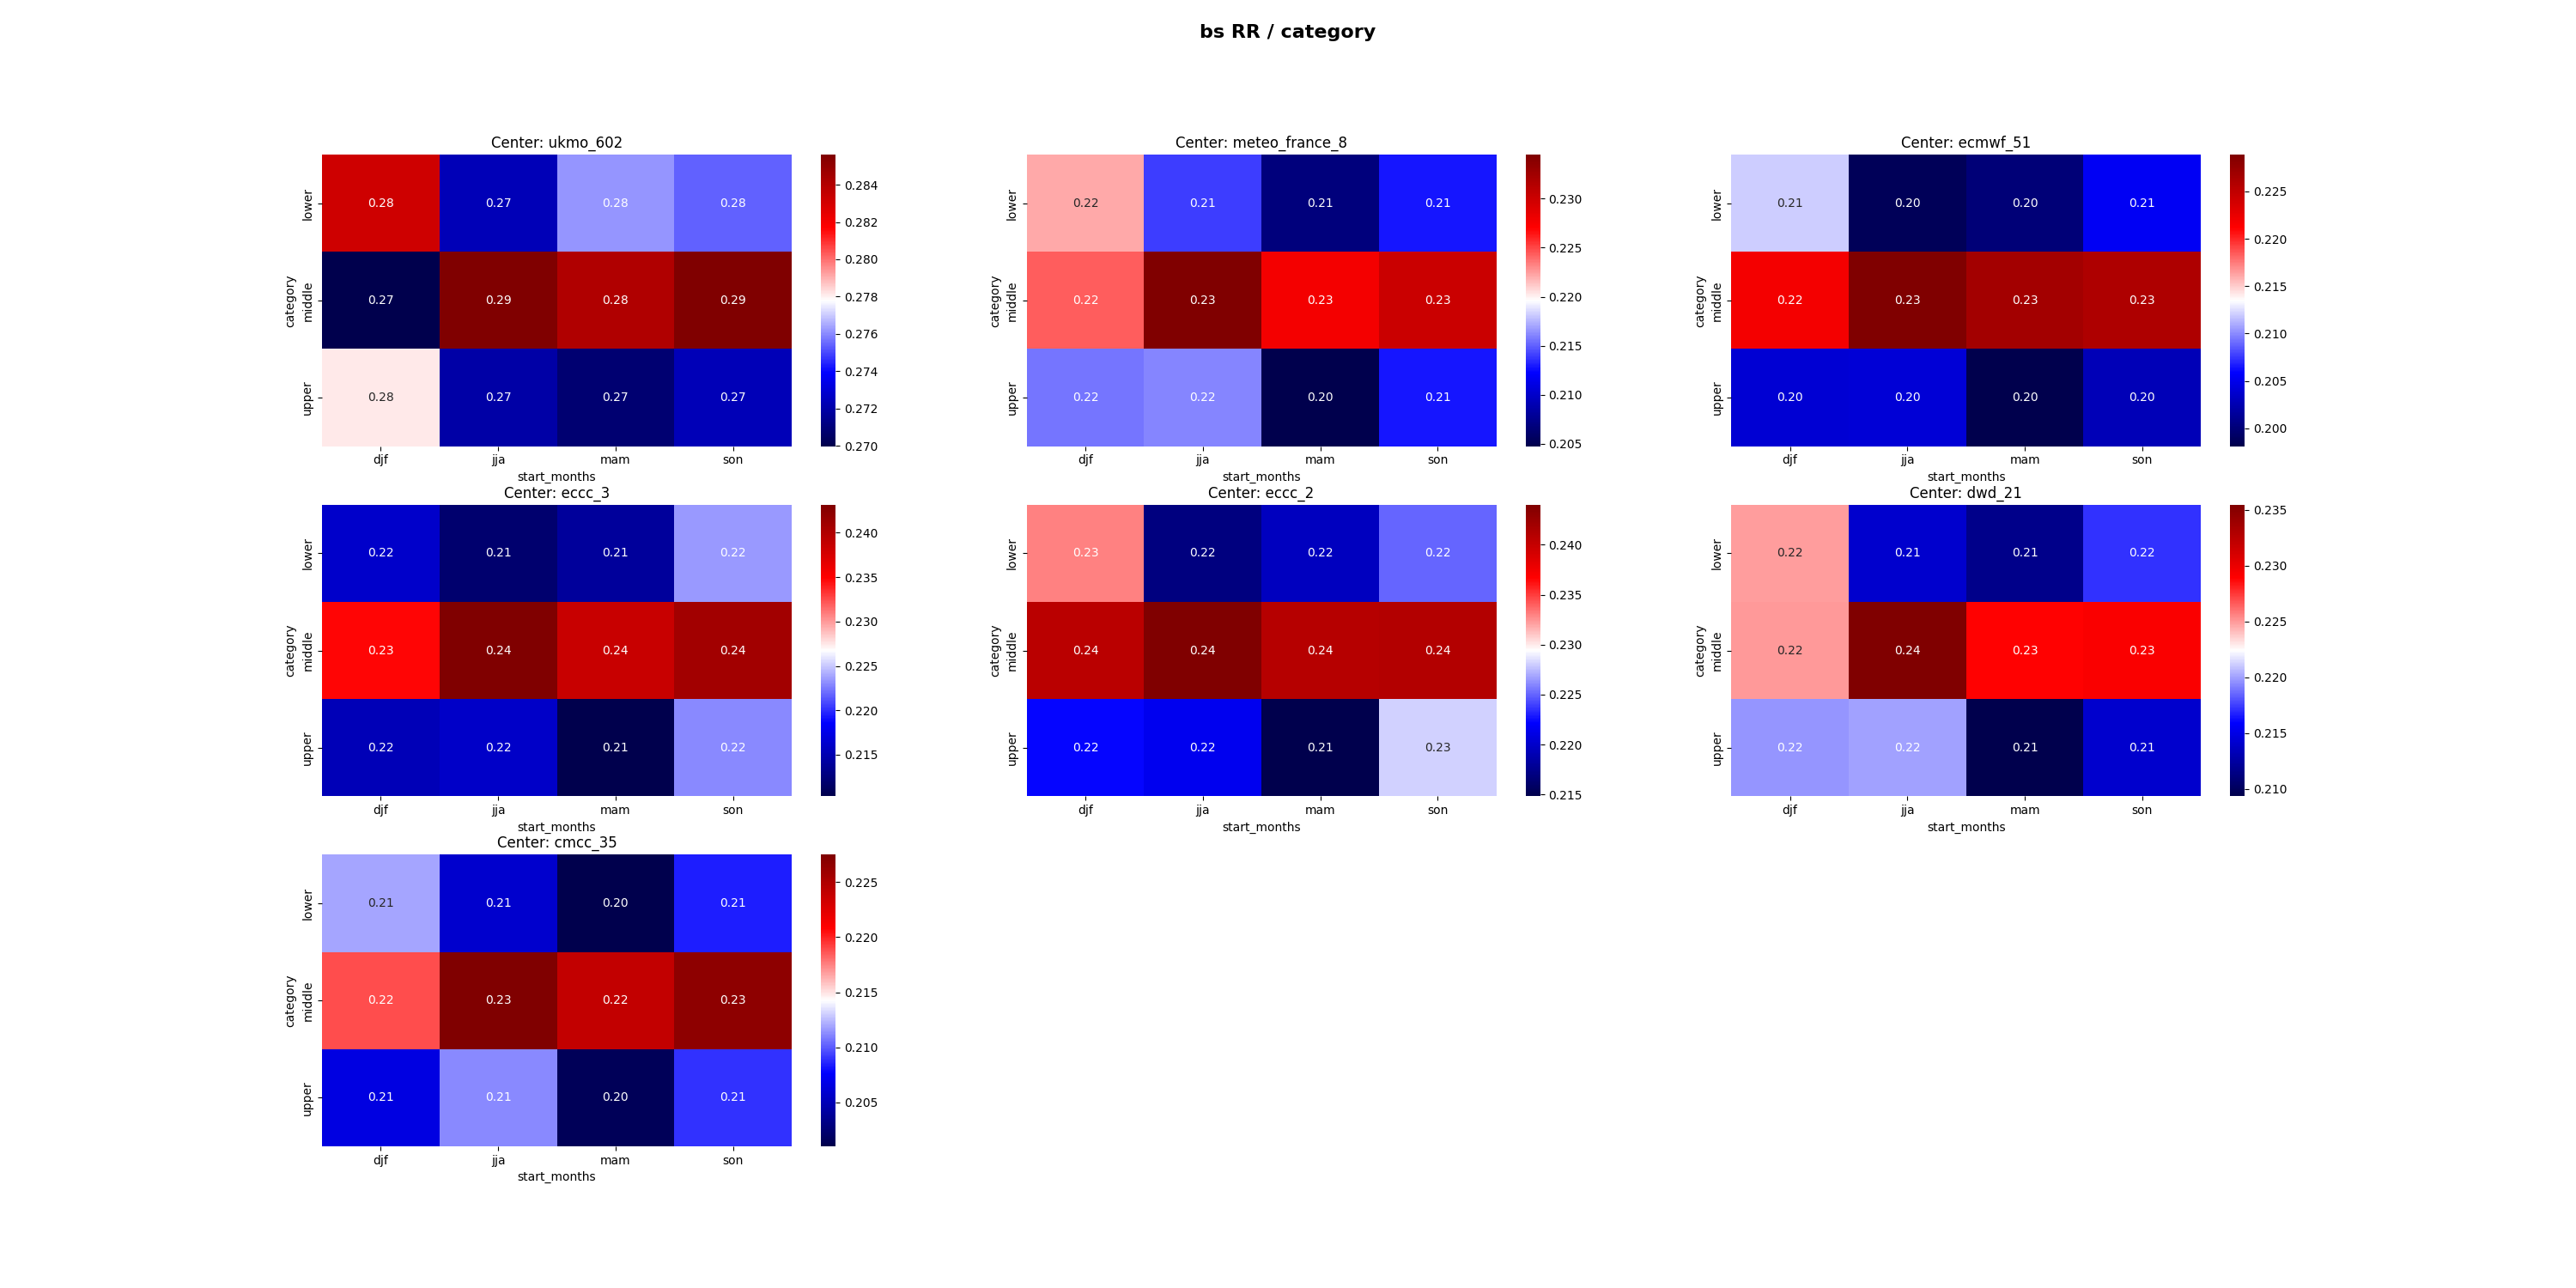
\includegraphics[scale=0.3]{bs_RR_category.png}
    \caption{The Brier Score for each category  . \textbf{\textit{(0 represents perfect BS)}}}
\end{figure}

we see in the figure above that Météo-France, ECMWF,DWD and CMCC35 are the best in Brier Score in the MENA region.





\begin{figure}[H]
    \centering
    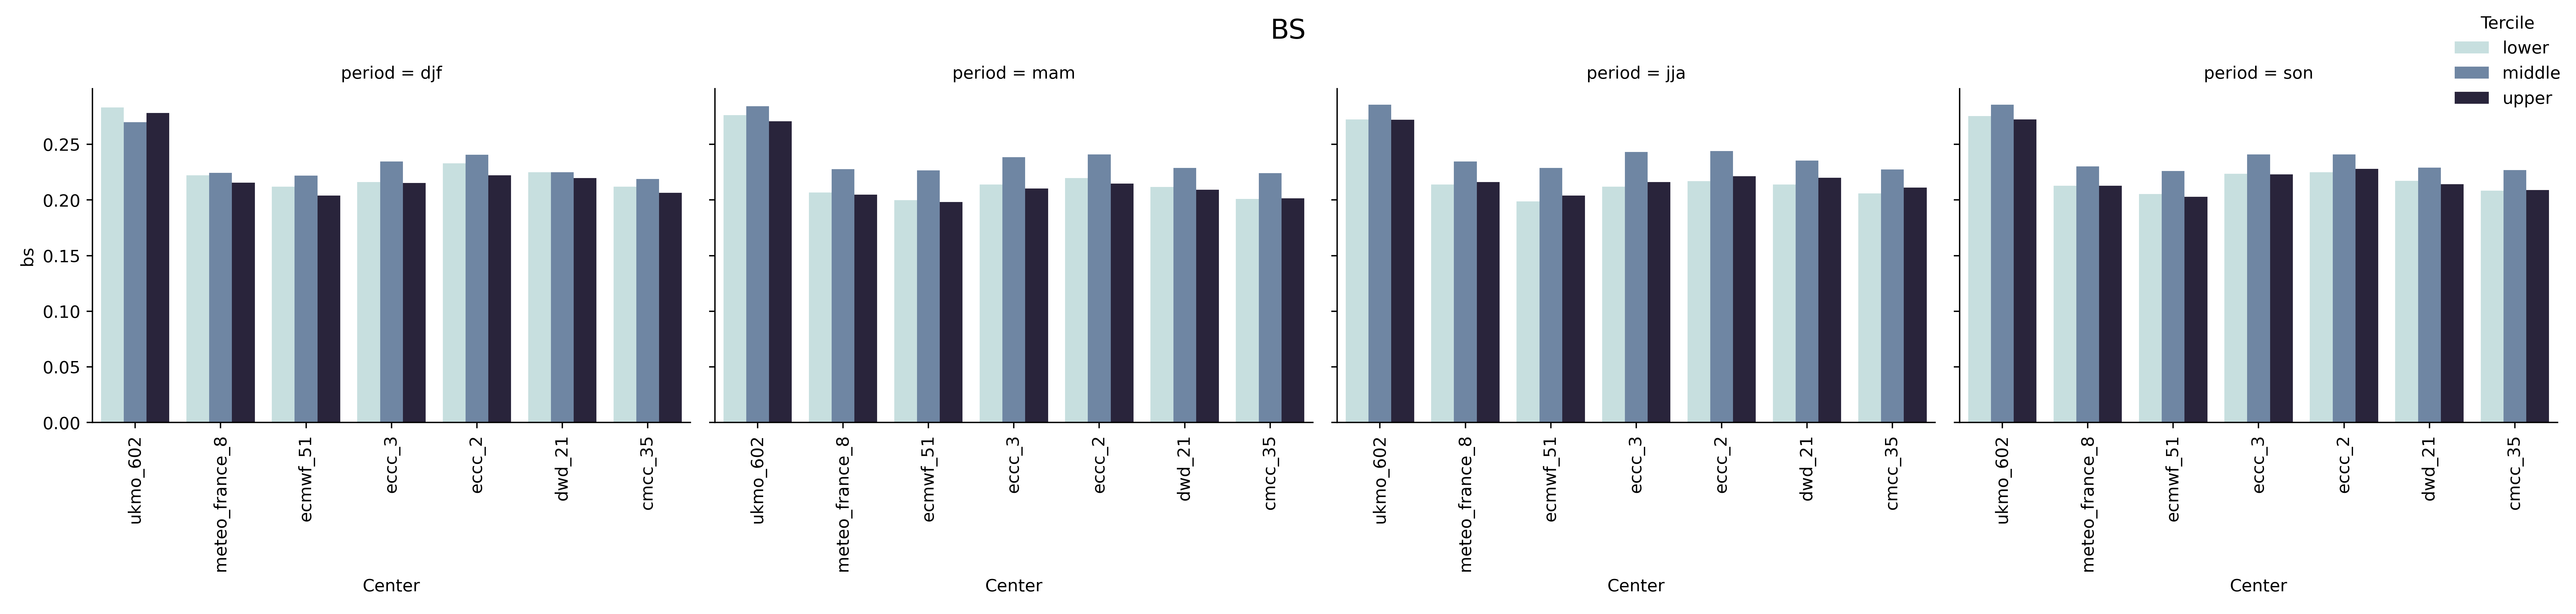
\includegraphics[scale=0.3]{bs.png}
    \caption{The average of  Brier Score on all categories    . \textbf{\textit{(0 represents perfect BS)}}}
\end{figure}
A deep analyze on each tercile category confirms the previous performance.



\subsubsection{Reliability}
the reliability\footnote{wmo guidance verification} measures the degree of correspondence between the forecast probability and the observed frequency for an event or outcome that is being predicted. It summarizes the conditional bias of the forecasts for a given event and is equal to the weighted average of squared differences between the forecast and conditional observed probabilities. If the reliability is 0, the forecast is perfectly reliable. To observe the frequency distribution, the forecast probability, from 0 to 1, is divided into 5 bins (0.1,0.3,0.5,0.7,0.9) to compare to the observed frequency in each of the same bin in this study. 
$$Reliability=\frac{1}{n} \sum\limits_{k=1}^{d} n_k(\bar{p_k}-\bar{y_k})^2$$
where:
\begin{itemize}
	\item $n_k$ is the number of forecasts for the $k_th$ probability value ($\bar{p_k}$)
	\item ($\bar{y_k}$) is the observed relative frequency for that value.
\end{itemize} 

\begin{figure}[H]
    \centering
    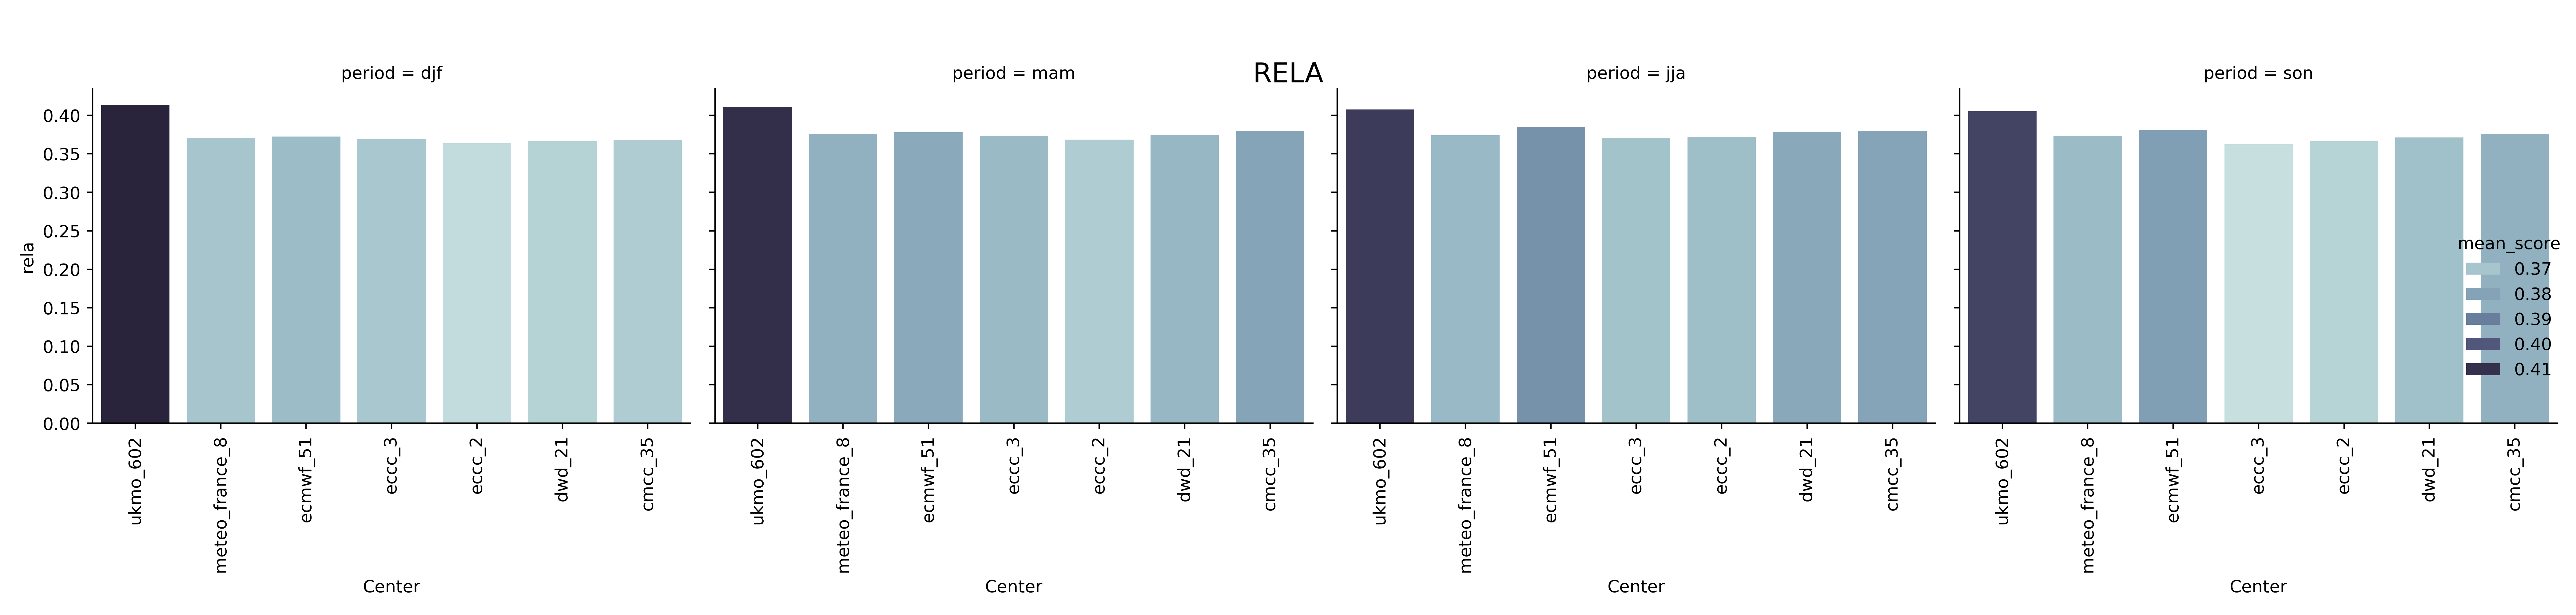
\includegraphics[scale=0.3]{rela_all.png}
    \caption{The Reliability Score  . \textbf{\textit{(0 means perfect Reliability)}}}
\end{figure}

In the figure above, all centers demonstrate similar performance.

\begin{figure}[H]
\centering
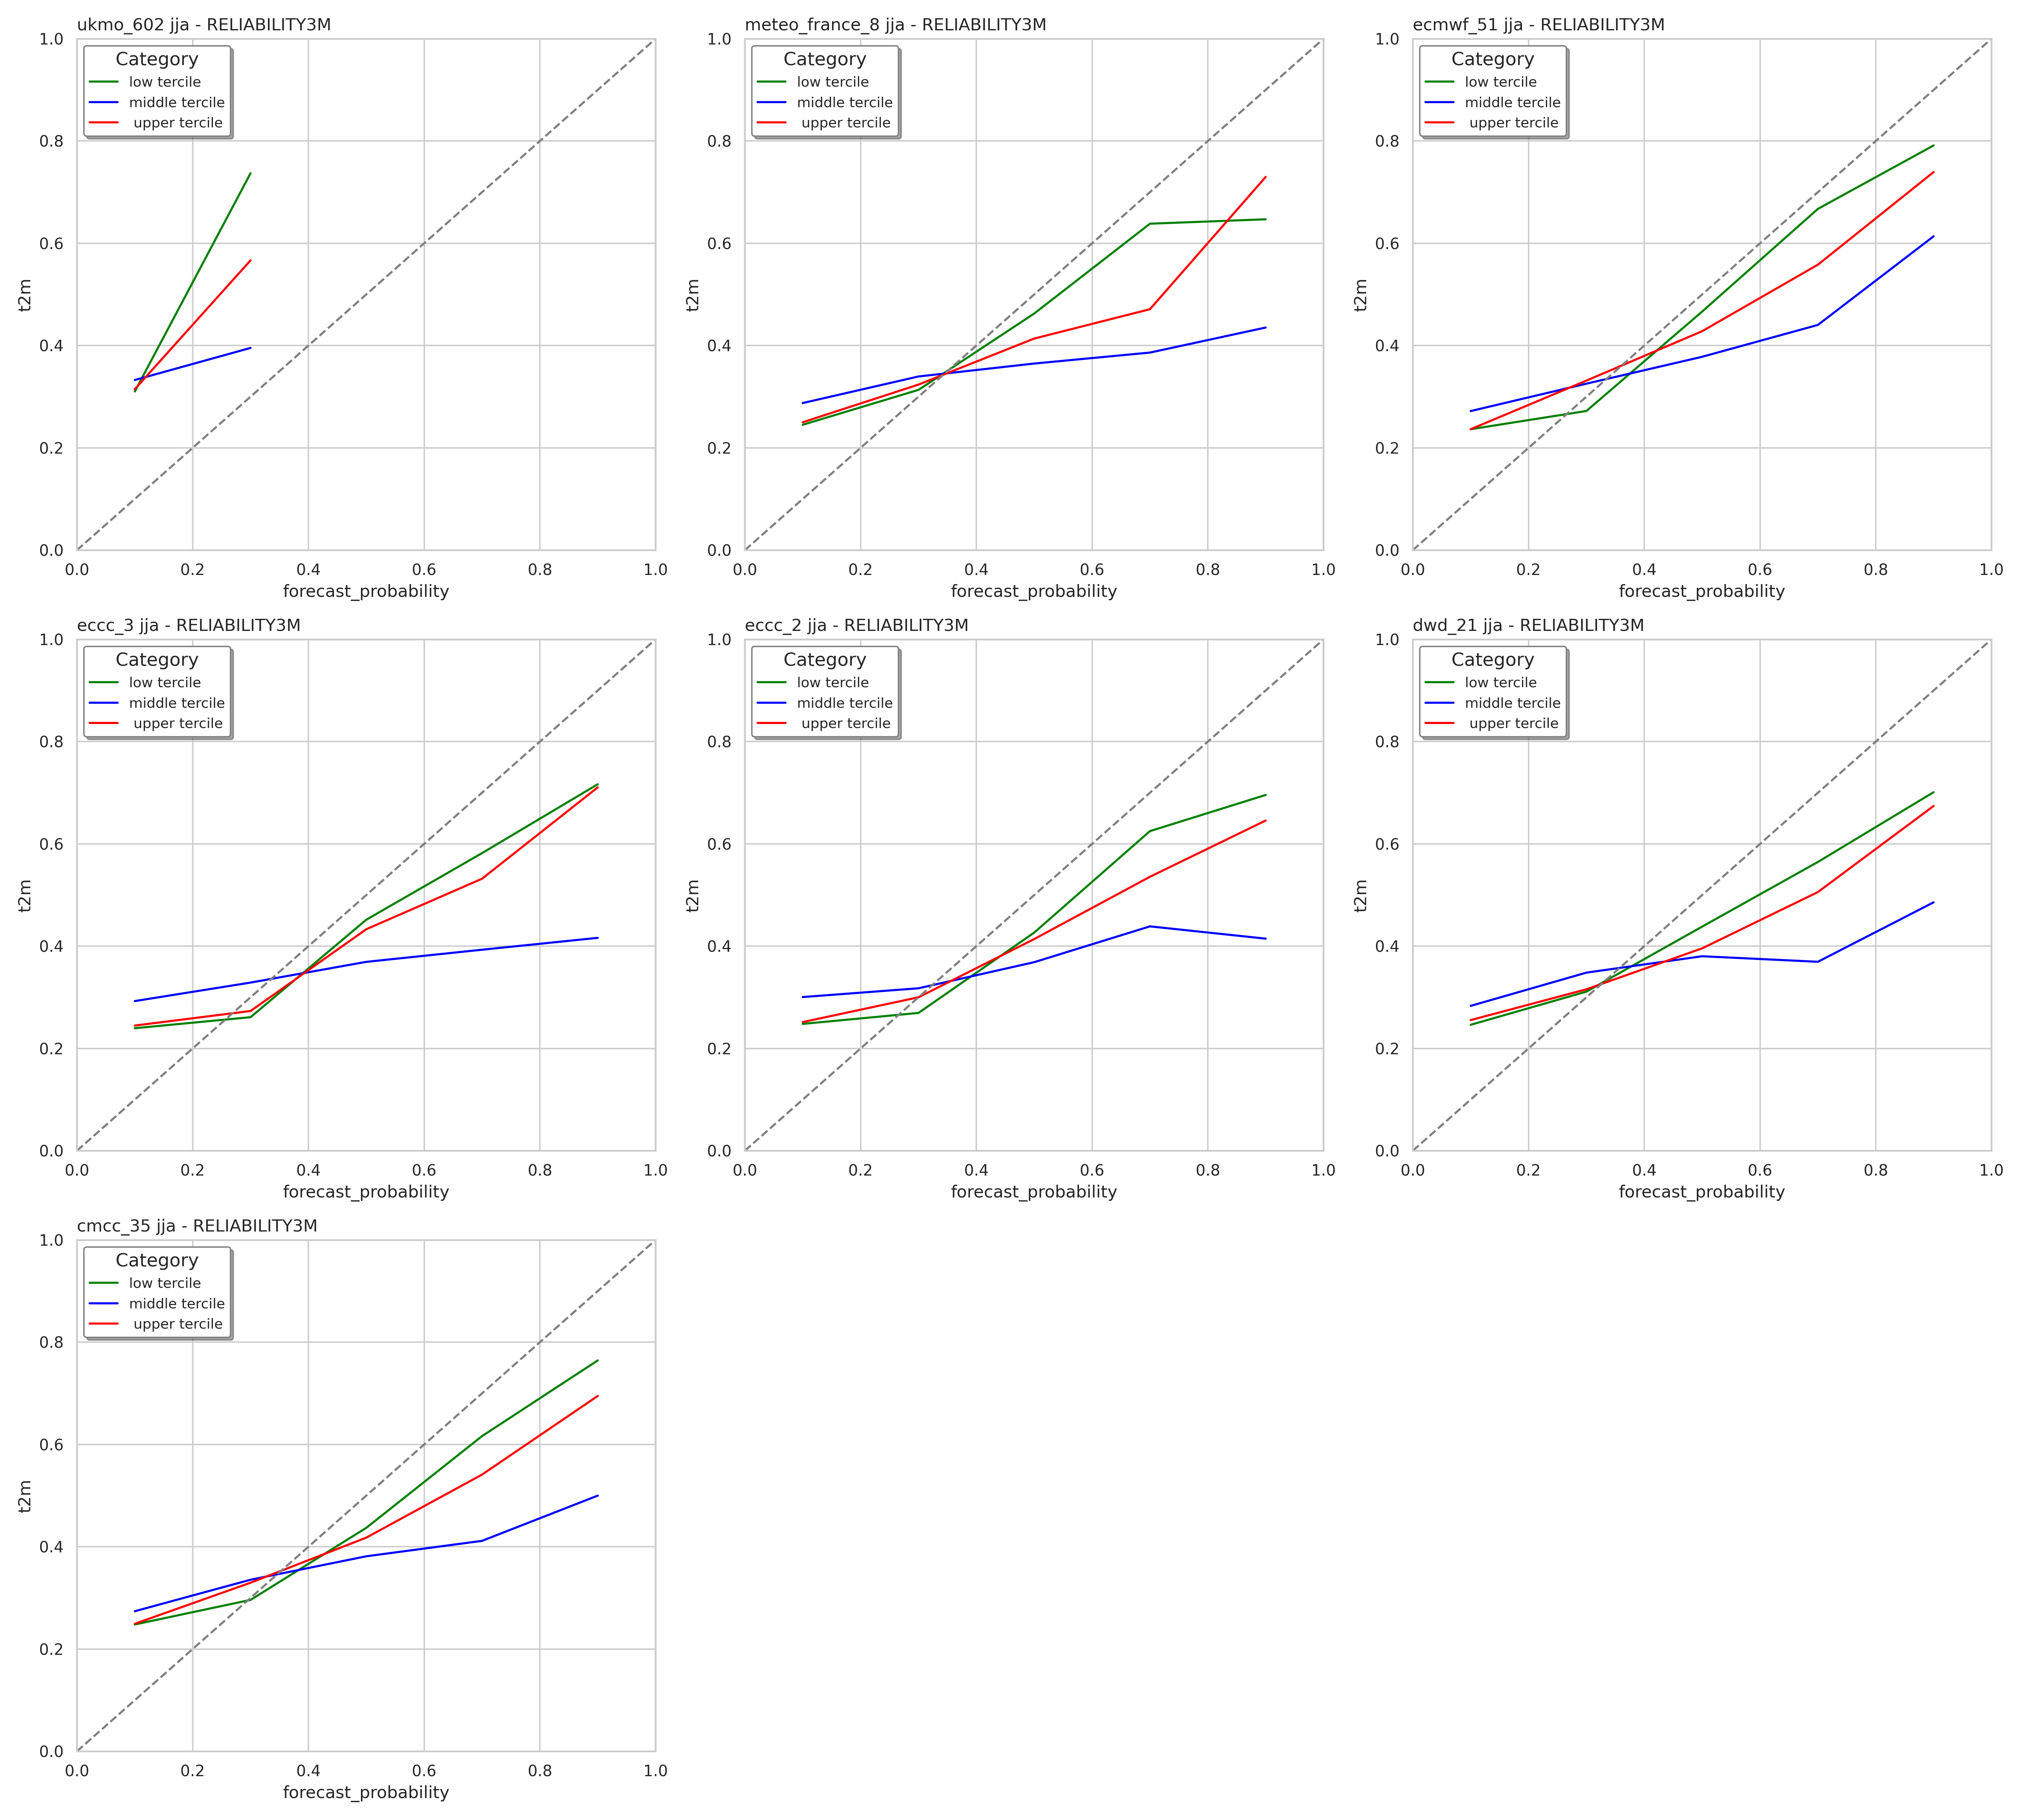
\includegraphics[scale=0.3]{rela_graphe.png}
\caption{The 3-month rolling mean for Reliability   . \textbf{\textit{Reliability is better in cases where the graphs are closer to the 45-degree line}}}
\end{figure}
for the 3-months rolling mean, the ECMWF has the best performance in reliability. The other centers have similar moderate performance, but the ukmo has poor reliability.







\subsubsection{The ranked probability score (RPS)}

The Ranked Probability Score (RPS) is a performance metric used in probabilistic forecasting to assess how well the predicted probability distribution matches the observed outcome distribution. It is particularly useful when there are multiple categories (e.g., terciles such as lower, middle, and upper) and is commonly applied in fields such as meteorology, climatology, and economics.

$$RPS=\frac{1}{n(m-1)}\sum\limits_{i=1}^{n} \sum\limits_{k=1}^{m-1} \left(\sum\limits_{j=1}^{k}(y_{j,i} - p_{j,i})\right)^2  $$

where : 

\begin{itemize}
	\item n is the number of forecasts.
	\item m is the number of categories.
	\item $y_{j,i}$ is 1 if the $i^th$ observation was in category j, and is 0 otherwise.
	\item $p_{j,i}$ is the $i^th$ forecast probability for category j
\end{itemize}

The score is the average squared “error” in the cumulative
probabilistic forecasts, and it ranges between 0\% for perfect forecasts (a probability of 100\%
was assigned to the observed category on each forecast) to a maximum of 100\% that can only
be achieved if all the observations are in the outermost categories, and if the forecasts are
perfectly bad (a probability of 100\% was assigned to the opposite outermost category to that
observed).


\begin{figure}[H]
    \centering
    \includegraphics[scale=0.3]{rps_RR_lead_time.png}
    \caption{The average of  RPS Score on all categories    . \textbf{\textit{(0 means perfect RPS)}}}
\end{figure}

\begin{figure}[H]
    \centering
    \includegraphics[scale=0.3]{rps_RR_category.png}
    \caption{The average of  RPS Score on all categories    . \textbf{\textit{(0 means perfect RPS)}}}
\end{figure}

In the figure above, all centers demonstrate similar performance, except for UKMO, which shows noticeably lower performance.





\subsubsection{Relative operating characteristics}
The ROC\footnote{wmo guidance verification} can be used in forecast verification to measure \textbf{\textit{the ability of the forecasts to distinguish an event from a non-event}}. For seasonal forecasts with three or more categories, the first
problem is to define the “event”. One of the categories must be selected as the current category
of interest, and an occurrence of this category is known as an event. An observation in any of
the other categories is defined as a non-event and no distinction is made as to which of these
two categories does occur. So, for example, if below normal is selected as the event, normal
and above normal are treated equally as non-events.

the score indicates the probability of successfully
discriminating below-normal observations from normal and above-normal observations. It
indicates how often the forecast probability for below normal is higher when below normal
actually does occur compared to when either normal or above normal occurs.


\begin{figure}[H]
    \centering
    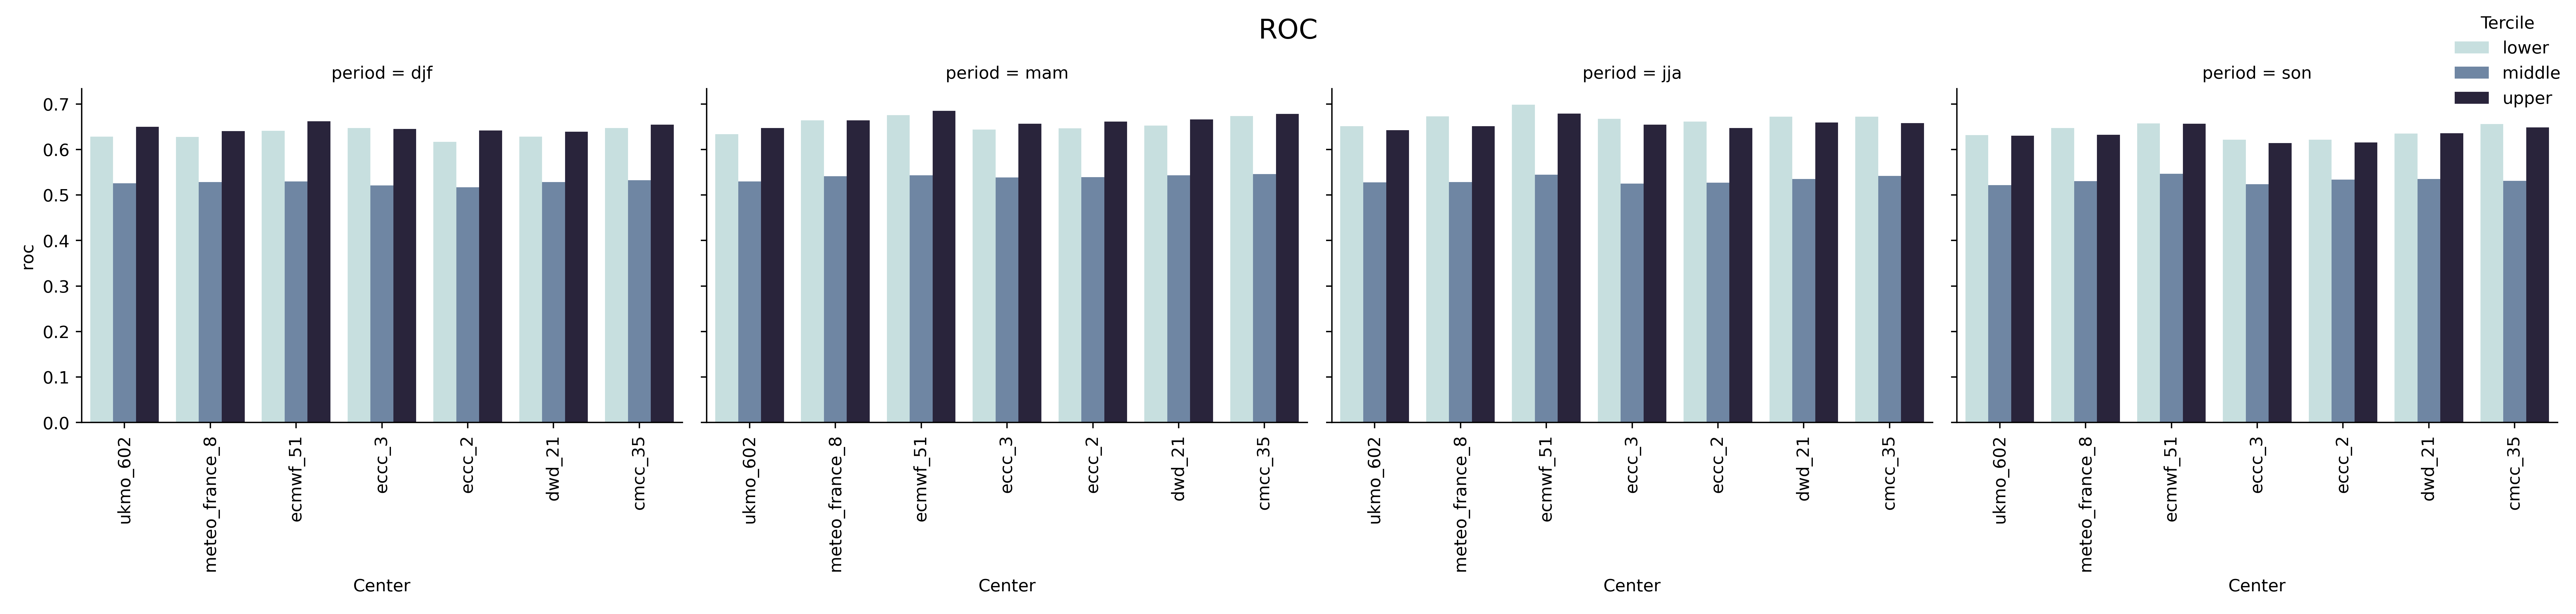
\includegraphics[scale=0.3]{roc.png}
    \caption{The ROC Score for each category  . \textbf{\textit{(1 means perfect ROC)}}}
\end{figure}

In the figure above, it is evident that all centers exhibit similar performance levels. However, the middle tercile consistently achieves the lowest score.
\begin{figure}[H]
    \centering
    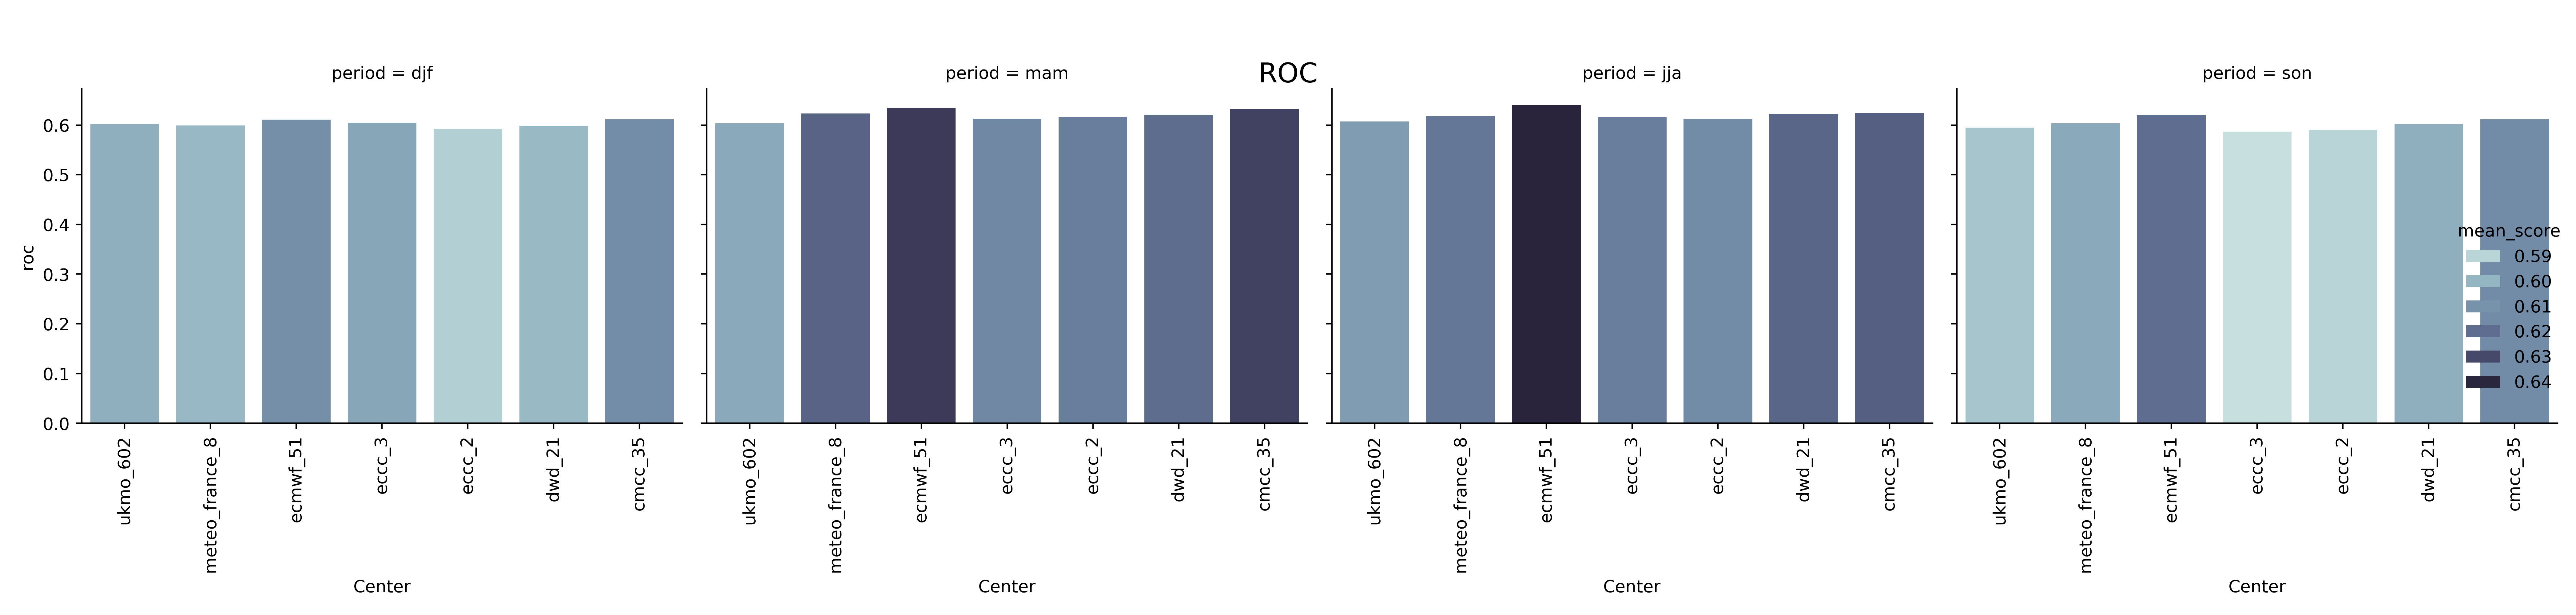
\includegraphics[scale=0.3]{roc_all.png}
    \caption{The average of  ROC Score on all categories    . \textbf{\textit{(1 means perfect ROC)}}}
\end{figure}


\begin{figure}[H]
    \centering
    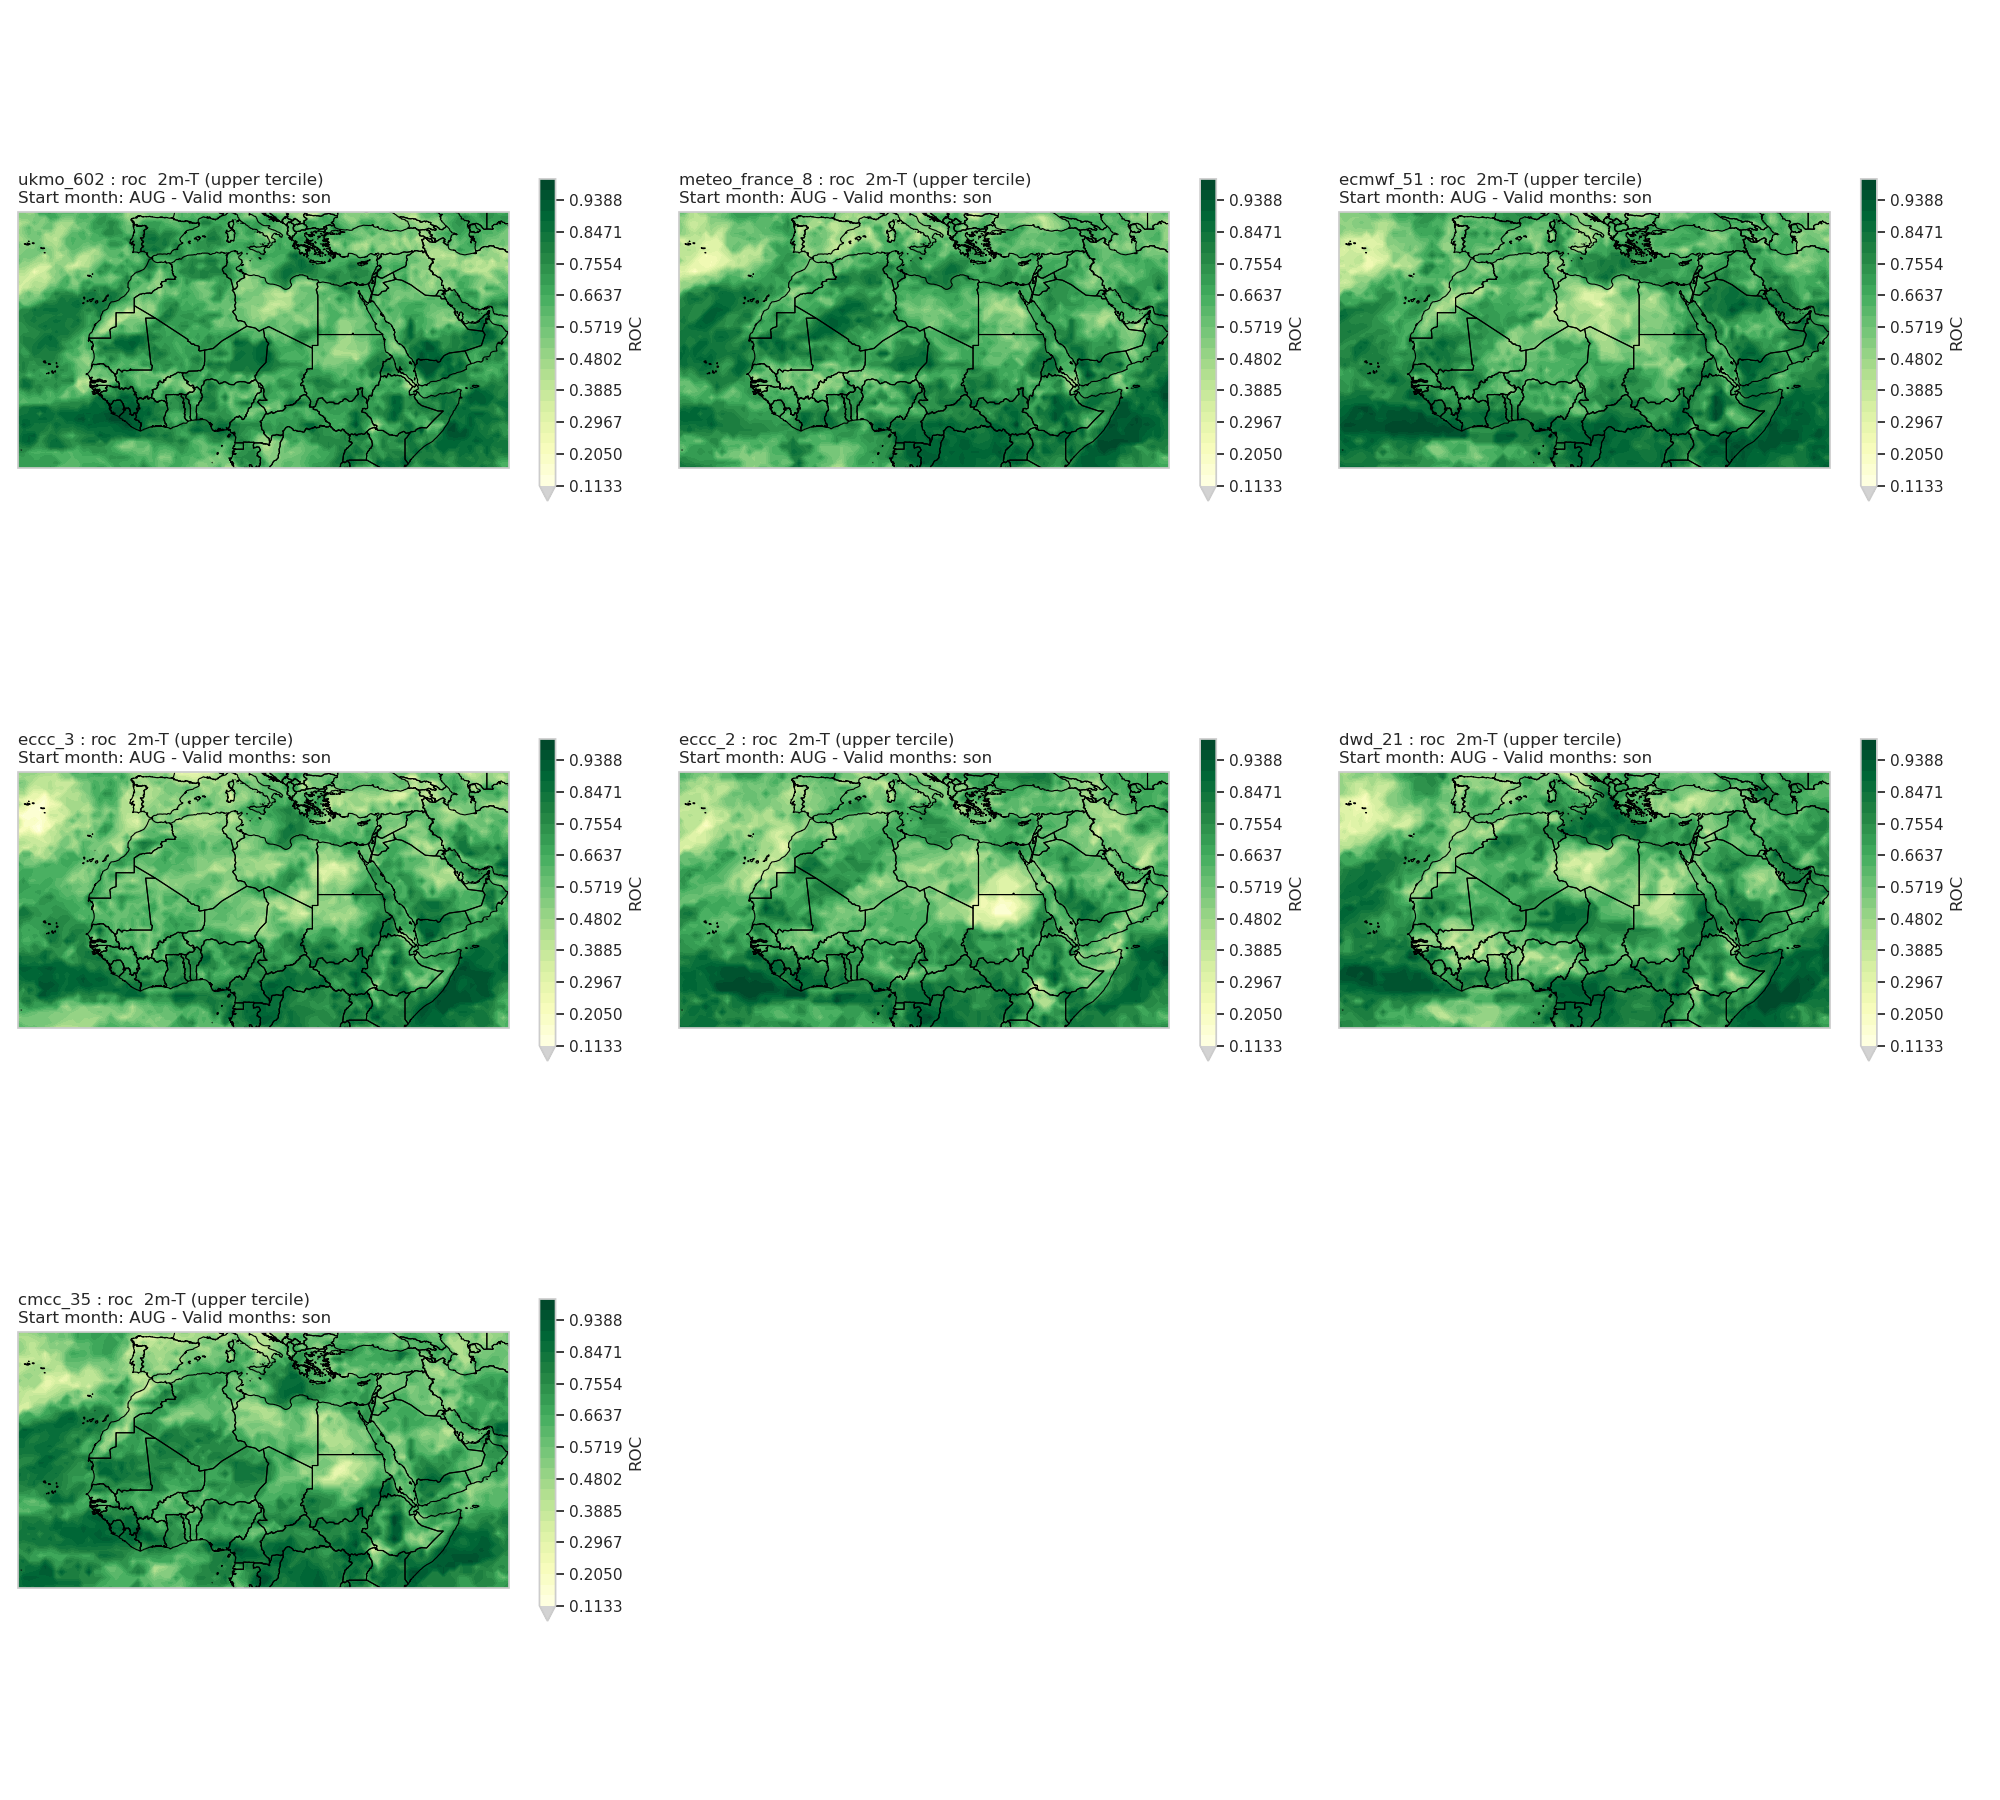
\includegraphics[scale=0.3]{ROC_UPPER_SON.png}
    \caption{The ROC Score Upper tercile SON    . \textbf{\textit{(1 means perfect ROC)}}}
\end{figure}


\subsubsection{Relative operating characteristics Skill Score}
The Relative Operating Characteristic Skill Score (ROCSS) is a measure used in forecast verification to assess the ability of probabilistic forecasts to discriminate between events and non-events. It builds on the Relative Operating Characteristic (ROC) curve, which plots the hit rate (true positive rate) against the false alarm rate (false positive rate) at various forecast probability thresholds.

\begin{itemize}
	\item The ROC curve evaluates the discrimination capability of a forecast, i.e., how well the forecast can separate occurrences of an event (e.g., below-normal temperature) from non-events (e.g., normal or above-normal temperature).
	\item The ROC Skill Score quantifies the area under the ROC curve (AUC) and compares it to a no-skill forecast.
\end{itemize}

	$$ROCSS=\frac{AUC-AUC_{no-skill}}{1-AUC_{no-skill}}$$
where:
\begin{itemize}
	\item $AUC$ : Area Under the ROC Curve for the forecast being evaluated.
	\item $AUC_{no-skill}$ : Area Under the Curve for a no-skill forecast 0.5 for our case.
\end{itemize}

Interpretation of ROCSS:
\begin{itemize}
	\item 1: Perfect discrimination ability.
	\item 0: No skill (forecast performs no better than random guessing).
	\item Negative values: Forecast performs worse than random guessing.
\end{itemize}
	

In the figure above, it is evident that the ECMWF exhibit the best performance for all terciles and periods. HOwever, we should notice that the performance is very bad for the middle tercile in all centers.

\begin{figure}[H]
    \centering
    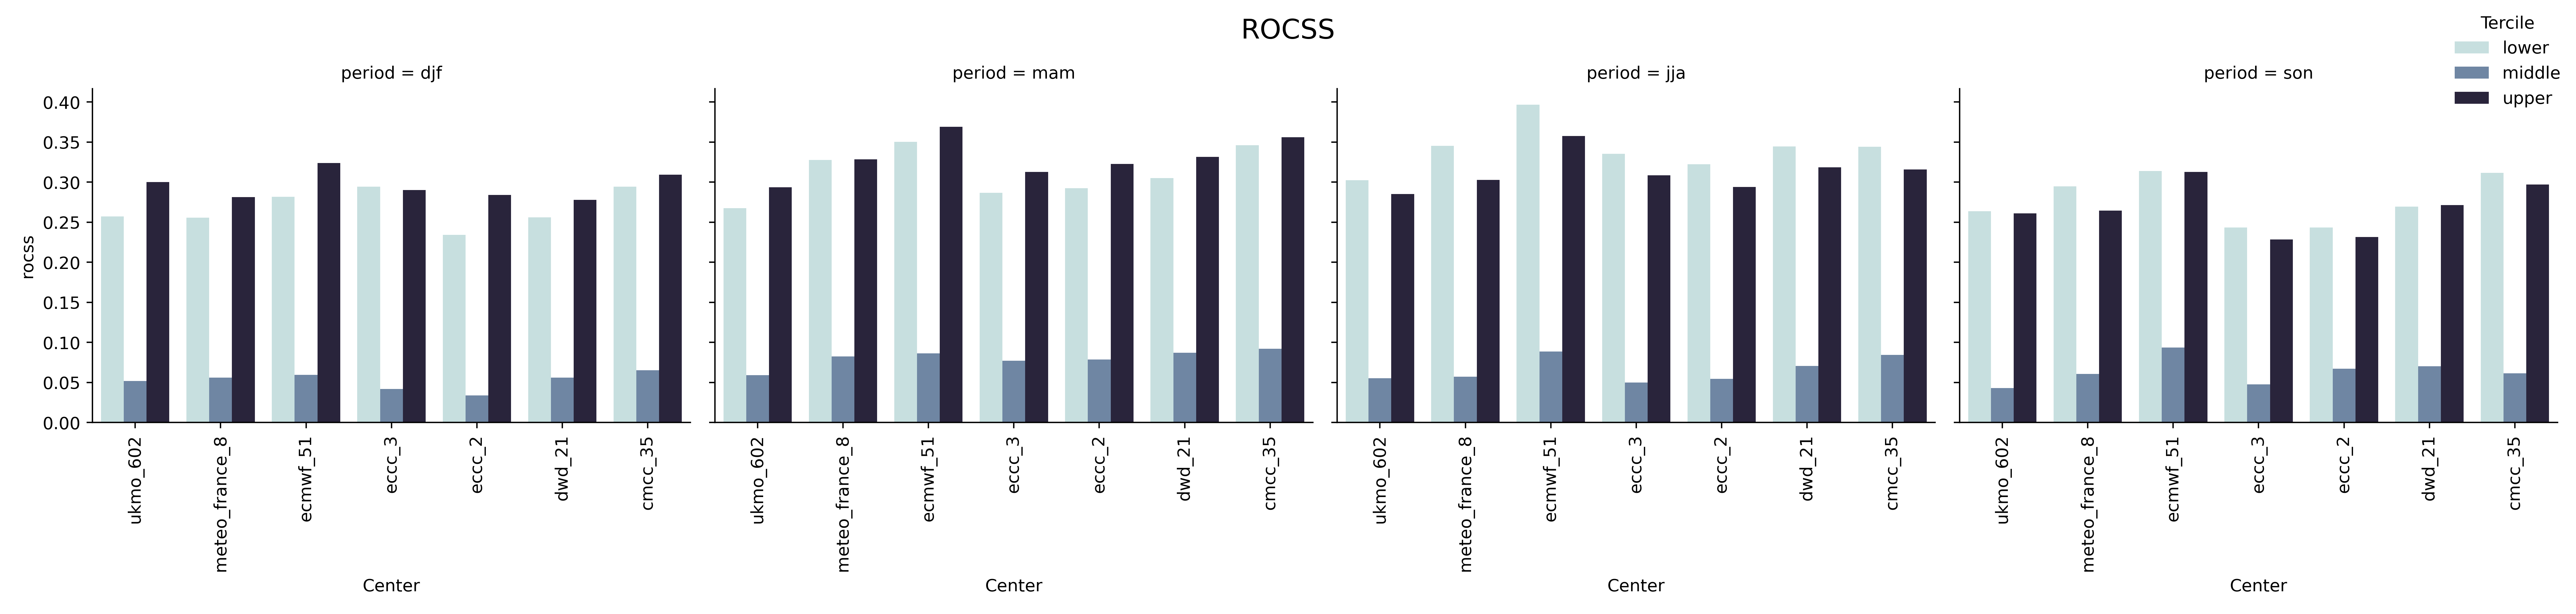
\includegraphics[scale=0.3]{rocss.png}
    \caption{The ROCSS Score for each category  . \textbf{\textit{(1 means perfect ROCSS)}}}
\end{figure}


\begin{figure}[H]
    \centering
    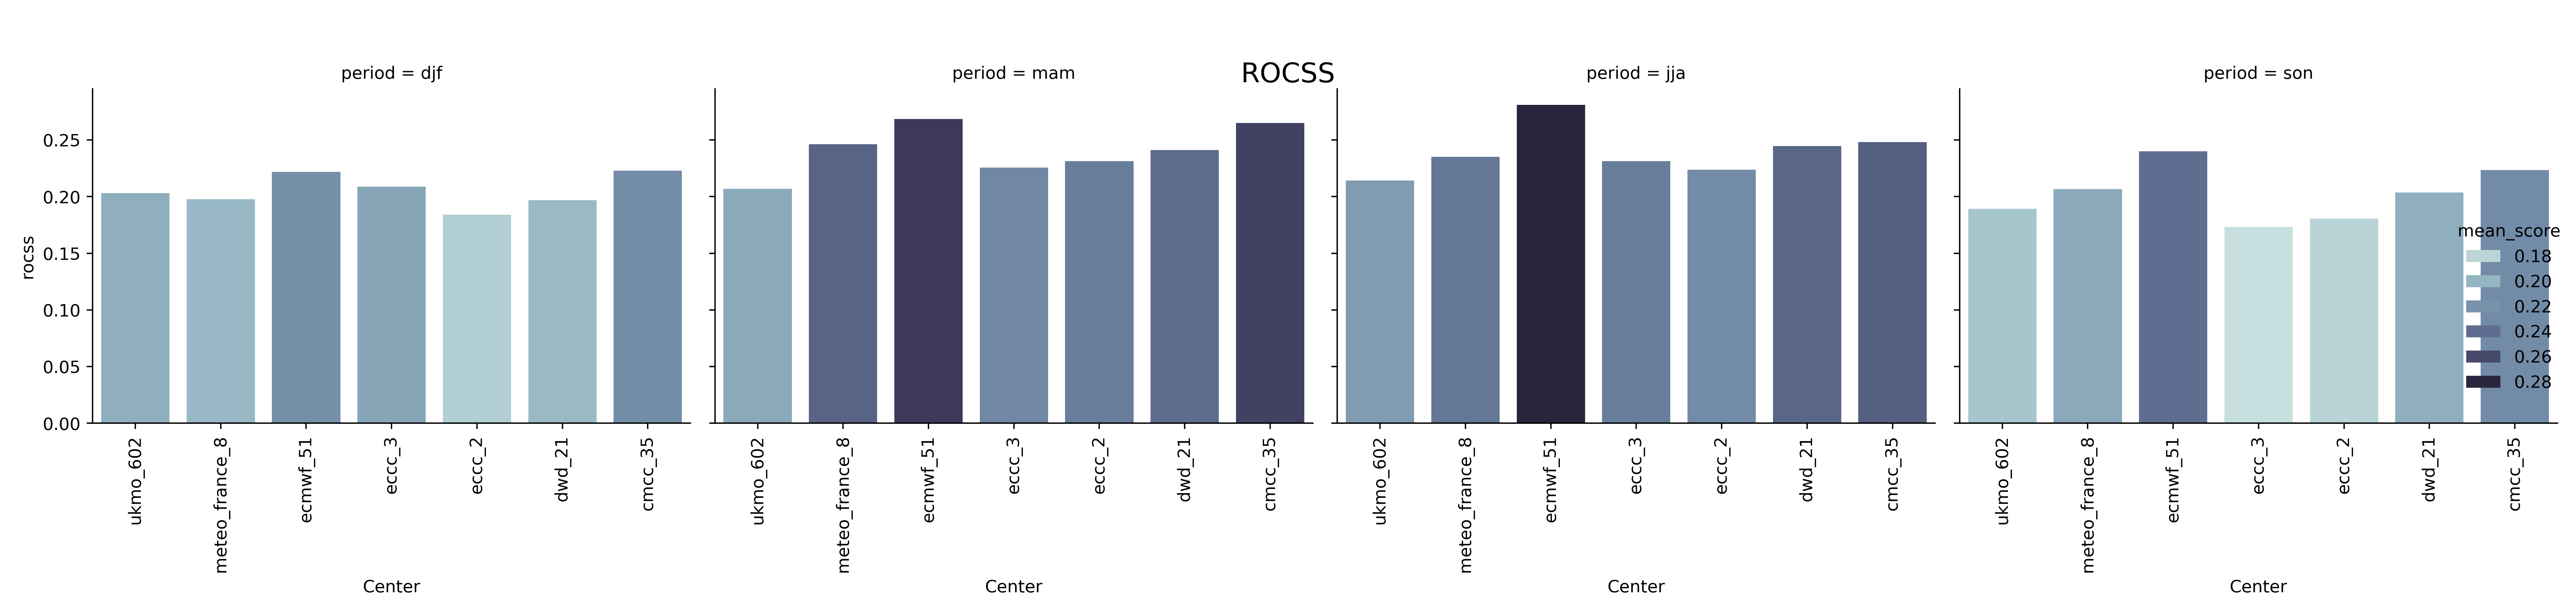
\includegraphics[scale=0.3]{rocss_all.png}
    \caption{The average of  ROCSS Score on all categories    . \textbf{\textit{(1 means perfect ROCSS)}}}
\end{figure}


\begin{figure}[H]
    \centering
    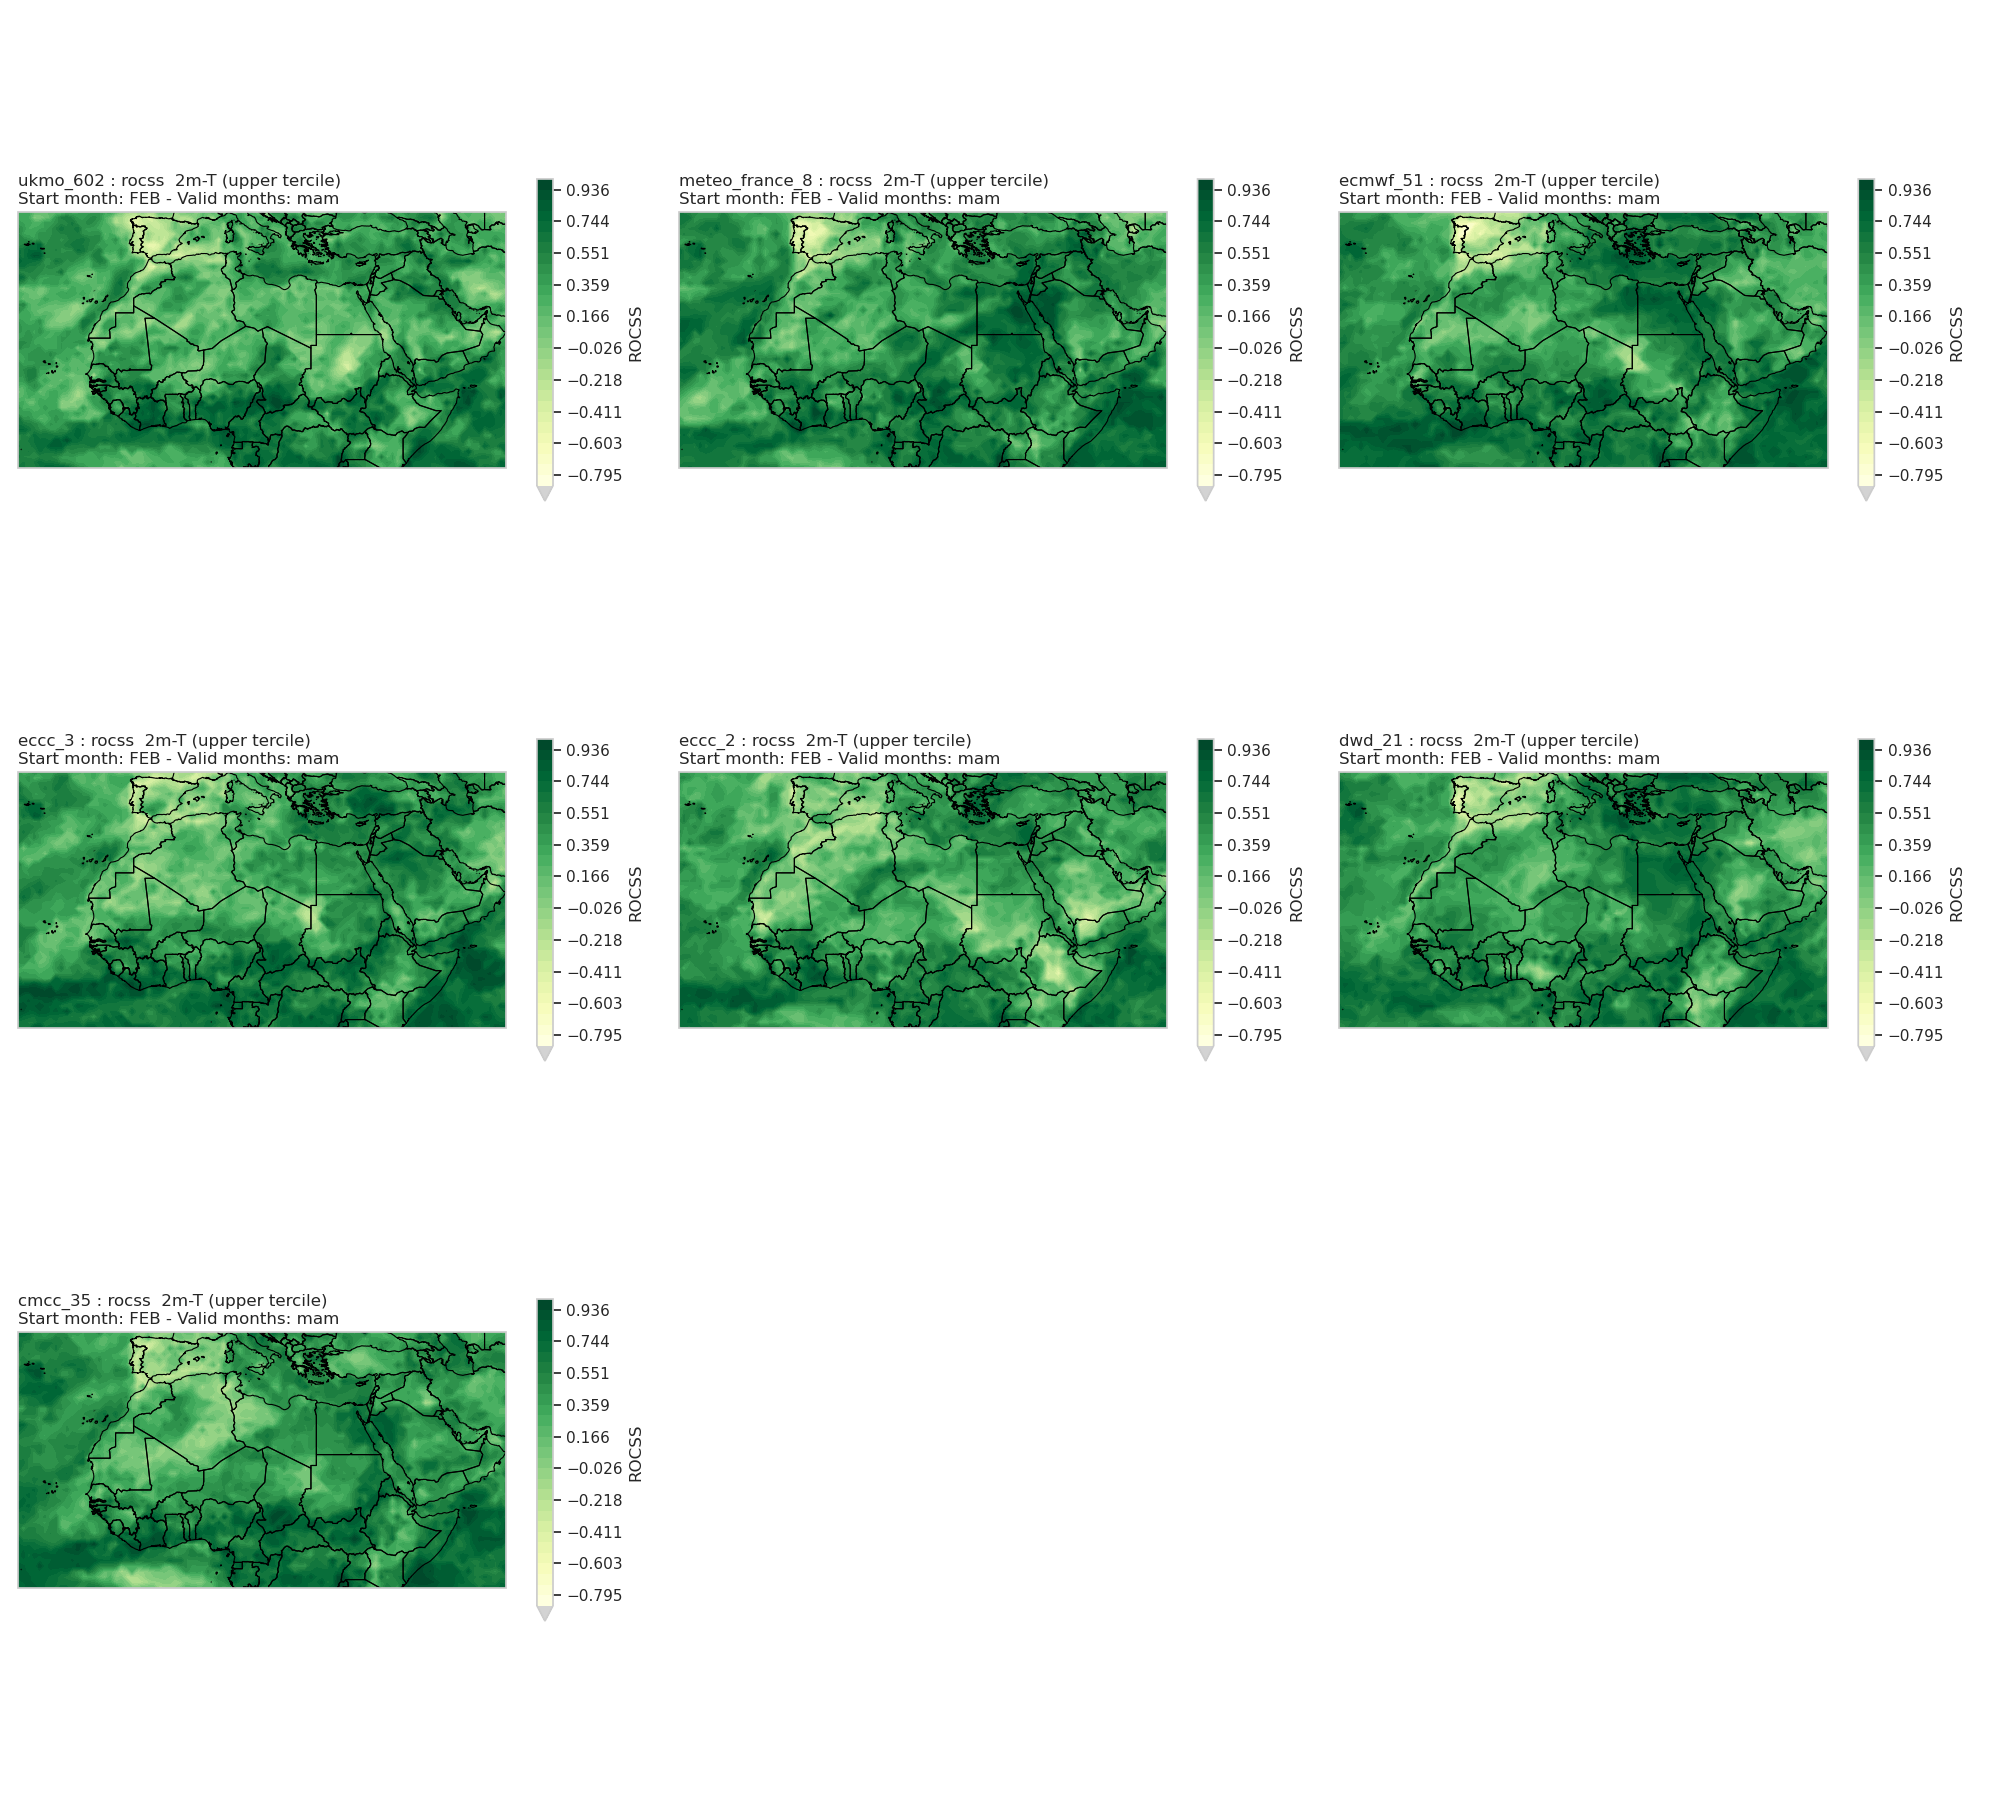
\includegraphics[scale=0.3]{ROCSS_MAM_UPPER.png}
    \caption{The ROC Skill Score Upper tercile MAM    . \textbf{\textit{(1 means perfect ROC)}}}
\end{figure}








\subsubsection{summary}
\begin{table}[h!]
\centering
\begin{tabularx}{\textwidth}{@{}p{2.5cm}p{4cm}p{4cm}p{2.5cm}p{3cm}@{}}
\toprule
\textbf{Metric}       & \textbf{Focus}                                    & \textbf{What it Measures}                         & \textbf{Dependent on Observed Outcomes?} & \textbf{Visualization/Tools}             \\ \midrule
\textbf{Reliability}   & Probabilities match observed frequencies          & Calibration of probabilities                      & Yes                                      & Reliability diagram                      \\
\textbf{Discrimination} & Differentiating between outcomes                 & Ability to distinguish events from non-events    & Yes                                      & ROC curve, AUC                           \\
\textbf{Sharpness}     & Boldness of probabilities (away from average)     & Confidence of the forecast                        & No                                       & Histogram of forecast probabilities      \\
\textbf{Resolution}    & Informativeness and variability of forecast       & Ability to provide specific, useful info         & Yes                                      & Brier Score decomposition                \\ \bottomrule
\end{tabularx}
\caption{Key differences between reliability, discrimination, sharpness, and resolution in seasonal forecasting.}
\label{tab:forecast_metrics}
\end{table}

\newpage
\thispagestyle{empty}
\mbox{}